\chapter{Aesthetic ideals in programming practices}
\label{chap:ideals}

The first step in our study of aesthetic standards in source code will identify the aesthetic ideals ascribed by programmers to the source code they write and read; that is, the syntactic qualifiers and semantic fields that they refer to when discussing program texts. To that end, we first start by clarifying whom we refer to by the term \emph{programmers}, revealing a multiplicity of practices and purposes, from \emph{ad hoc}, one-line solutions, to printed code and massively-distributed codebases.

We then turn to the kinds of beauty that these programmers aspire to. After expliciting our methodology of discourse analysis, we engage in a review of the various kinds of publications and writings that programmers write, read and refer to when it comes to qualifying their practice. From this will result a cluster of adjectives which we see being used in an aesthetic manner. These will provide an empirical basis when examining, in subsequent chapters, the formal arrangements of program texts.

From these, we can then move to a description of which aesthetic fields are being referenced by programmers on a broader level, and consider how multiple kinds of beauties, from literary, to architectural and scientific conceptions of beauty can overlap and be referred to by the same medium.

Finally, we conclude this chapter by elaborating on one of the points of overlap in these different references: the importance of function, craft and knowledge in the disposition and representation of code. We will show how this particular way of working  plays a central role in an aesthetic approach to source code and results from the specificity of code as a cognitive material, a specificity we will focus on in the next chapter.

\pagebreak

\section{The practice of programmers}

The history of software development is that of a specific, reserved practice which was born in the aftermath of the second world war, which trickled down to broader and broader audiences at the eve of the twenty-first century. Through this development, various paradigms, platforms and applications have been involved in producing software, resulting in different epistemic communities and communities of practice \citep{cohendet_organisational_2001}, in turn producing different types of source code. Each of these focus on the description of specific instructions to the computer, but do so with particular characteristics. To this end, we take a socio-historical stance on the field of programming, highlighting how diverse practices emerge at different moments in time, how they are connected to contemporary technical and economic organizations, and for specific purposes.

Even though such types of reading and writing source code often overlap with one another, this section will highlight a diversity of  ways in which code is written, notably in terms of origin—how did such a practice emerge?—, references—what do they consider good?—, purposes—what do they write for?—and examples—how does their code look like?. First, we take a look at the software industry, to identify professional \emph{software developers}, the large code bases they work on and the specific organizational practices within which they write it. They are responsible for the majority of source code written today, and do so in a professional and productive context, where maintainability, testability and reliability are the main concerns. Then, we turn to a parallel practice, one that is often exhibited by software developers, as they also take on the stance of \emph{hackers}. Disambiguating the term reveals a set of practices where curiosity, cleverness, and idiosyncracy are central, finding unexpected solutions to complex problems, sometimes within artificial constraints. Finally, we look at \emph{scientists} and \emph{poets}. On one end, \emph{scientists} embody a rather academic approach,  focusing on abstract concepts such as simplicity, minimalism and elegance; they are often focused on theoretical issues, such as mathematical models, as well as programming language design, but are also involved in the implementation of algorithms. On the other end, \emph{poets} read and write code first and foremost for its textual and semantic qualities, publishing code poems online and in print, and engaging deeply with the range of metaphors allowed by this dynamic linguistic medium.

While this overview encompasses most of the programming practices, we leave aside some approaches to code, mainly because they do not directly engage with the representation of source code as a textual matter. More and more, end-user applications provide the possibility to program in rudimentary ways, something referred to as the "low-code" approach \citep{team_lowcode_2021}, and thus contributing to the blurring of boundaries between programmers and non-programmers\footnote{For instance, Microsoft's Visual Basic for Applications, Ableton's Max For Live, MIT's Scrath or McNeel's Grasshopper are all programming frameworks which are not covered within the scope of this study. In the case of VBA and similar office-based high-level programming, it is because such a practice is a highly personal and \emph{ad hoc} one, and therefore is less available for study.}.

\subsection{Software developers}
\label{subsec:software-developers}
\subsubsection{From local hardware to distributed software}

As Niklaus Wirth puts it, \emph{the history of software is the history of growth in complexity} \citep{wirth_brief_2008}, while paradoxically, a lowering of the barrier to entry. As computers' technical abilities in memory managment and processing power increased year on year since the 1950s, the nature of writing instructions shifted as well.

In his history of the software industry, Martin Campbell-Kelly traces the development of a discipline through an economic and a technological lens, and he identifies three consecutive waves in the production of software \citep{campbell-kelly_airline_2003}. During the first period, as soon as the 1950s, and continuing throughout the 1960s, software developers were contractors hired to engage directly with a specific computing machine. These computing, mainframes, were large, expensive, and rigid machines, requiring hardware-specific knowledge of the corresponding Assembler instruction set, since they didn't yet feature an operating system which could facilitate some of the more basic memory allocation and input/output functions, and thus enable interoperable program-writing\footnote{One of the first operating systems, MIT's Tape Director, would be only developped in 1956 \citep{ross_personal_1986}}. Two distinct groups of people were involved in the operationalization of such machine: electrical engineers, tasked with designing hardware, and programmers, tasked with implementing the software. While the former historically received the most attention \citep{ross_personal_1986}, the latter was mostly composed of women and, as such, not considered essential in the process \citep{light_when_1999}. At this point, then, programming remains closely tied to hardware.

The second period in software development starts in the 1960s, as hardware switched from vacuum tubes to transistors and from magnetic core memory to semiconductor memory, making them faster and more capable to handle complex operations.  On the software side, the development of several programming languages, such as FORTRAN, LISP and COBOL, started to address the double issue of portability—having a program run unmodified on different machines with different instruction sets—and expressivity—allowing programmers to use high-level, English-like syntax, rather than assembler instruction codes. By then, programmers are no longer theoretically tied to a specific machine, and therefore acquire a certain autonomy, a recognition which culminates in the naming of the field of \emph{software engineering} in 1968 at a NATO conference \citep{randell_nato_1996}.

The third and final phase that Campbell-Kelly identifies is that of mass-market production: following the advent of the UNIX family of operating systems, the distribution of the C programming language, the wide availability of C compilers, and the appearance of personal computers such as the Commodore 64, Altair and Apple II, software could be effectively entirely decoupled from hardware\footnote{For a more detailed account of the personal computer revolution, see: Cerruzzi, P., A History of Modern Computing \citep{ceruzzi_history_2003}}. And yet, despite this growth in popularity, software immediately enters a crisis: software development projects run over time and budget, prove to be unreliable in production and unmaintainable in the long-run. The creation of software is no longer a corollary to the design of hardware, and as an independent field would as such become the main focus of computing as a whole \citep{ceruzzi_history_2003}. It is at this time that discussions around best practices in writing source code started to emerge, once the activity of the programmer was no longer restricted to \emph{tricks by means of which he contrived to squeeze the impossible into the constraints of his equipment} \citep{dijkstra_humble_2007}.

This need for a more formal approach to the actual process of programming found one of its most important manifestations in Edsger Djikstra's \emph{Notes on Structured Programming} \citep{dijkstra_chapter_1972}. In it, he argues for moving away from programming as a craft, and towards programming as an organized discipline, with its methodologies and systematization of program construction. Despite its laconic section titles\footnote{See, for instance, Chapter 1: "\emph{On our inability to do much}"}, Djikstra's 1972 report nonetheless contributed to establish a more rigorous typology of the constructs required for reliable, provable programs—based on fundamental heuristics such as sequencing, selection, iteration and recursion—, and aimed at the formalization of the practice. Along with other subsequent developments (such as Hoare's contribution on proper data structuring \citep{hoare_chapter_1972}, or the rise of object-oriented programming with Smalltalk) programming would solidify its foundations as a profession:

\begin{quote}
  We knew how the nonprofessional programmer could write in an afternoon a three-page program that was supposed to satisfy his needs, but how would the professional programmer design a thirty-page program in such a way that he could really justify his design? What intellectual discipline would be needed? What properties could such a professional programmer demand with justification from his programming language, from the formal tool he had to work with?  \citep{dijkstra_chapter_1972}
\end{quote}

As a result of such interrogations comes an industry-wide search for solutions to the intractable problem of programming: that it is \emph{a technique to manage information which in turn produces information}. To address such a conundrum, a variety of tools, formal methods and management processes enter the market; they aim at acting as a \emph{silver bullet} \citep{brooks_mythical_1975}, addressing the cascade of potential risks\footnote{See \url{https://catless.ncl.ac.uk/Risks/} for such risks} which emerge from large software applications. However, this growth in complexity is also accompanied by a diversification of software applications: as computers become more widely available, and as higher-level programming languages provide more flexibility in their expressive abilities, software engineering engages with a variety of domains, each of which might need a specific solution, rather than a generic process. Confronted with this diversity of applications, business literature on software practices flourishes, being based on the assumption that the complexity of software should be tackled at its bottleneck: the reading and writing of source code.

The most recent step in the history of software developers is the popularization of the Internet and of the World Wide Web. Even though the former had existed under as ArpaNet since 1969, the network was only standardized in 1982 and access to it was provided commercially in 1989. Built on top of the Internet, the latter popularized global information exchange, including technical resources to read and write code. Software could now be written by remote individual written on \emph{cloud computing} platforms, shared through public repositories and deployed via containers with a lower barrier to entry than at the time of source code printed in magazines, of overnight batch processing and of non-time-sharing systems.

Software developers have written some of the largest codebases to this date, since this type of activity represents the most significant fraction of programmers. Due to its close ties to commercial distributors, however, source code written in this context often falls under the umbrella of proprietary software, thus made unvailable to the public. Some examples that we include in our corpus are either professional codebases that have been leaked\footnote{Such as the Microsoft Windows XP source code \citep{warren_windows_2020}.}, open-source projects that have come out of business environments, such as Soundcloud's Prometheus, Kirby's CMS System, Facebook's React, or large-scale open-source projects which nonetheless adhere to structured programming guidelines, such as Donald Knuth's TeX typesetting system or the Linux Foundation's Linux kernel.

\subsubsection{Features of the field}

The features of these codebases hint at the qualities that software developers have come to ascribe to their object of practice. First, the program texts they write are large, much larger than any other codebase included in this study. They often feature multiple programming languages and are highly structured and standardized: each file follows a pre-established convention in programming style, which favors an authoring by multiple programmers without any obvious trace to a single individual authorship. These program texts stand the closest to a programming equivalent of engineering, with its formalisms, standards and usability. From this perspective, the IEEE's Software Engineering Body of Knoweldge (SWEBOK) provides a good starting point to survey the specificities of software developers as source code writers and readers \citep{bourque_swebok_2014}; the main features of which include the definition of requirements, design, construction, testing and maintenance.

Software requirements are the acknowledgement of the importance of the \emph{problem domain}, the domain to which the software takes its inputs from, and to which it applies its outputs. For instance, software written for a calculator has arithmetic as its problem domain; software written for a learning management system has students, faculty, education and courses as its problem domain; software written a banking institution has financial transactions, savings accounts, fraud prevention and credit lines as its problem domain. Requirements in software development aim at formalizing as best as possible the elements that must be used by the software in order to perform a successful computation, and an adequate formalization is a fundamental requirement for a successful software application.

Subsequent to the identification and codification of requirements, software design relates to the overall organization of the software components, considered not in their textual implementation, but in their conceptual agency. Usually represented through diagrams or modelling languages, it is concerned with \emph{understanding how a system should be organized and designing the overall structure of that system} \citep{sommerville_software_2010}. Of particular interest is the relationship that is established between software development and architecture. Considered a creative process rather than a strictly rational one, due to the important role of the contexts in which the software will exist (including the problem domain) \citep{sommerville_software_2010}, software architecture operates both from a top-down perspective, laying down an abstract blueprint for the implementation of a system, as well as form a bottom-up one, representing how the different components of an existing system interact. This apparent contradiction, and the role of architecture in the creative aspects of software development, will be further explored in section \ref{sec:aesthetic-domains} below.

Software construction relates to the actual writing of software, and how to do so in the most reliable way possible. The SWEBOK emphasizes first and foremost the need to minimize complexity\footnote{Following Hoare's assessment in his Turing Award Lecture that \emph{"there are two ways of constructing a software design: one way is to make it so simple that there are obviously no deficiencies, and the other way is to make it so complicated that there are no obvious deficiencies."}}, in anticipation of likely changes and possible reuse by other software systems. Here, the emphasis on engineering is particularly salient: while most would refer to the creation of software as \emph{writing} software, the IEEE document refers to it as \emph{constructing} software\footnote{The term software construction refers to the detailed creation of working software through a combination of coding, verification, unit testing, integration testing, and debugging. \citep{bourque_swebok_2014}.}. Coding is only assessed as a practical consideration, one which should not take up the most attention, if the requirements, design and testing steps are satisfyingly implemented.

In parallel, a whole field of business litterature \citep{martin_clean_2008,hendrickson_software_2002,fowler_refactoring_1999,mcconnell_code_2004} has focused specifically on the process of writing code, starting from the assumption that:

\begin{quote}
  We will never be rid of code, because code represents the details of the requirements. At some level those details cannot be ignored or abstracted; they have to be specified. And specifying requirements in such details that a machine can execute them is \emph{programming}. \citep{martin_clean_2008}
\end{quote}

As we see in these two perspectives on the role that code should play, the tension identified by Djikstra some thirty years before between craft and discipline is still alive and well at the beginning of the twenty-first century, even though the attention paid to code still relates to the need for reliability and maintainability in a maturing industry.

Software maintenance, finally, relates not to the planning or writing of software, but to its reading. Software is notoriously filled with bugs\footnote{McConnell estimates that the industry average is about 15 - 50 errors per 1000 lines of delivered code. \citep{mcconnell_code_2004}.} and can, at the same time, be easily fixed while already being in a production environment through software update releases. This means that the lifecycle of a software doesn't stop when then first version is written, but rather when it does not run anywhere anymore. The nature of software allows for it to be edited across time and space, by other programmers which might not have access to the original group of implementers: consequently, software should be first and foremost understandable—SWEBOK lists the first feature of coding as being \emph{techniques for creating understandable source code} \citep{bourque_swebok_2014}. This requirement ties back to one of the main problems of software, which is its notorious cognitive complexity, one that remains at any stage of its development.

\vspace{1\baselineskip}

What does this look like in practice, then? Ideals of clarity, reusability and reliability—and their opposites—can be found in some of the available code bases of professional software. The paradox to be noted here is that, even though software developers write the most code, it is the least accessible online and, as such, the following excerpts are covering the range of commercial software (Microsoft Windows), licensed and publicly available software (Kirby).

The first excerpts come from the source code for Microsoft Windows 2000, which was made public in 2004. The program text contains  28,655 files, the largest of our  corpus, by multiple orders of magnitude, with 13,468,327 combined lines and including more than 10 different file extensions. Taking a closer look at some of these files allow us to identify some of the specific features of code written by software developers, and how they specifically relate to architectural choices, collaborative writing and verbosity.

First, the most striking visual feature of the code is its sheer size. Representing such a versatile and low-level system such as an operating system manifest themselves in files that are often above 2000 lines of code. In order to allow abstraction techniques at a higher-level for the end-developer, the operating system needs to do a significant amount of "grunt" work, relating directly to the concrete reality of the hardware platform which needs to be operated. For instance, the initialization of strings of text for the namespaces (a technique directly related to the compartmentalization) is necessary, repetitive work which can be represented using a rhythmic visual pattern, such as in the \lstinline{cmdatini.c} source file, reproduced partially in \ref{code:ms2000}.

\begin{listing}
  \inputminted[fontsize=\footnotesize, breaklines, breakanywhere]{c}{./corpus/ms2000.c}
  \caption{Unicode string initialization in Microsoft 2000 operating system}
  \label{code:ms2000}
\end{listing}

The repetition of the \lstinline{RtlInitUnicodeString} call in the first part of this listing stands at odds with today's industry-standard practices of not repeating oneself; a standard only adhered to in the second part of the code, the two \lstinline{for()} statements. While this practice would only be formalized in Andy Hunt's \emph{The Pragmatic Programmer} in 1999 \citep{hunt_pragmatic_1999}, the longevity of the windows 2000 operating system and its update cycle would nonetheless have affected how this code is written. The reason why such a repetition applies is the requirement of registering each string with the kernel. Dealing with a different problem domain (kernel instructions) leads to a different kind of expected aesthetics\footnote{Effectively, references to \lstinline{RtlInitUnicodeString()} happen 1580 times across 336 files}.

Verbosity, the act of explicitly writing out statements which could be functionally equivalent in a compacted form, is a significant feature of the Windows 2000 codebase, and also relies on a particular semantic environment: that of using the C programming language. As mentioned above, the development of C and UNIX in the 1970s have led to wide adoption of the former, and to some extent of the later (even though Windows is a notable exception since it is an operation system not based on the UNIX tradition). What we see in this listing is the consequence of this development: using a verbose language results in a verbose program text, something we will see in the following section on hacker's code and will explore much further in chapter 5.

Another significant aesthetic feature of the Windows 2000 program text is its use of comments, and specifically how those comments representing the multiple, layered authorship. This particular source code is one that is written across individuals and across time, each with presumably its own writing style. Yet, writing source code within a formal organization often implies the adoption of coding styles, with the intent that \emph{all code in any code-base should look like a single person typed it, no matter how many people contributed} \citep{waldron_idiomatic_2020}. For instance, the excerpt in \ref{code:buffer_c} from \lstinline{jdhuff.c} is a example of such overlapping of styles:

\begin{listing}
  \inputminted[fontsize=\footnotesize]{c}{./corpus/buffer.c}
  \caption{Programming styles overlapping in the source code of Microsoft 2000.}
  \label{code:buffer_c}
\end{listing}

Here, we see different writings of comments(using \lstinline{//} and \lstinline{/* */}) as well as  different kinds of capitalizations. Those comments are ignored at compile time: that is, they are not meaningful to the machine, and are only expected to be read by other programmers, and in this case primarily by programmers belonging to one's organization. This hints at the various origins of the authors, or at the very least at the different moments, and possible mental states of the potential single-author: irregularity in comment writing can connect to irregularities in semantic content of the comments. This irregularity becomes suspicious, and leads to ascribing a different epistemological value to them. If comments aren't procedurally guaranteed to be reflected in the execution, and outcome, of the program, then one tend to rely on the fact that "the only document that describes your code completely and correctly is the code itself" \citep{goodliffe_code_2007}. This excerpt highlights the constant tension between source code as the canonical origin of knowledge of what the program does and how it does it, while comments reflect the idiosyncratic dimension of all natural-language expressions of human programmers.

And yet, this chronological and interpersonal spread of the program text, combined with organizational practices, require the use of comments in order to maintain aesthetic and cognitive coherence in the program, if only by the use of comment headers, which locate a specific file within the greater architectural organization of the program text (see \ref{code:enum_c}).

\begin{listing}
  \inputminted{c}{./corpus/enum.c}
  \caption{pnpenum.c shows the traces of multiple authors collaborating on a single file over time.}
  \label{code:enum_c}
\end{listing}


This highlights both the multiple authorship (here, we have one original author and one revisor) as well as the evolution in time of the file: comments are the only manifestation of this layering of revisions which ultimately results in the "final" software\footnote{The term "final" is in quotes, since the Windows 2000 source contains the mention \lstinline{BUGBUG} 7436 times across 2263 files, a testament to the constant state of unfinishedness that software tends to remain in.}.

A complementary example is the Kirby CMS\footnote{Allgeier, Bastian et. al., \url{https://github.com/getkirby/kirby}, 2011, consulted in 2022}. With development starting in 2011 and a first release in 2012, it developed a steady userbase, correlated in Google Trends analytics\footnote{https://trends.google.com/trends/explore?date=all\&q=kirby\%20cms}, consistent forum posts\footnote{https://forum.getkirby.com} and commit history on the main repository\footnote{https://github.com/getkirby/kirby}. Kirby is an open-source, developer-first (meaning that it affords direct engagement of other developers with its architecture through modification, extension or partial replacement), single-purpose project. As such, it stands at the other end of the commercial, efficient software spectrum than Microsoft Windows 2000.

The Kirby source code is entirely available online, and the following snippets hint at another set of formal values—conciseness, expliciteness and delimitation. Conciseness can be seen in the lengths of the various components of the code base. For instance, the core of Kirby consists in 248 files, with the longest being \lstinline{src/Database/Query.php} at 1065 lines, and the shortest being \lstinline{src/Http/Exceptions/NextRouteException.php} at 16 lines, for an average of 250 lines per file (compared to the leading project in the field, Wordpress.org, which has respectively 3466 files, with the longest file comprising 9353 lines of code (\lstinline{customize-controls.js}), and the shortest 1line (such as \lstinline{script-loader-packages.php})\footnote{The project was cloned on 06.05.2022 from the official repository at \url{https://github.com/WordPress/WordPress}}).

If we look at a typical function declaration within Kirby, we found one such as the \lstinline{distinct()} setter for Kirby's database, reproduced in \ref{code:query_php}.

\begin{listing}
  \inputminted{php}{./corpus/query.php}
  \caption{Query.php}
  \label{code:query_php}
\end{listing}

Out of these 11 lines, the actual functionality of the function is focused on one line, \lstinline{$this->distinct = $distinct;}. Around it are machine-readable comment snippets, and a function wrapper around the simple variable setting. The textual overhead then comes from the wrapping itself: the actual semantic task of deciding whether a query should be able to include distinct select clauses (as opposed to only allowing join clauses), is now decoupled from its actual implementation (one could describe to the computer such an ability to generate distinct clauses by assigning it a boolean value, or an integer value, or passing it as an argument for each query, etc.). The quality of this writing, at first verbose, actually lies in its conciseness in relation to the possibilities for extension that such a form of writing allows: the \lstinline{distinct()} function could, under other circumstances, be implemented differently, and still behave similarly from the perspective of the rest of the program. Additionally, this wrapping enables the setting of default values (here, \lstinline{true}), a minimal way to catch bugs by always providing a fallback case.

Kirby's source code is also interestingly explicit in comments, and succint in code. Let us take, for instance, from the \lstinline{Http\\Route} class (see \ref{code:route_php}).

\begin{listing}
  \inputminted{php}{./corpus/route.php}
  \caption{Route.php}
  \label{code:route_php}
\end{listing}

The 9 lines above the function declaration are machine-readable documentation. It can be parsed by a programmatic system and used as input to generate more classical, human-readable documentation\footnote{See, for instance, JavaDocs, or ReadTheDocs}. This is noticeable due to the highly formalized syntax \lstinline{param string name_of_var}, rather than writing out "this function takes a parameter of type string named \lstinline{name_of_var}". This does compensate for the tendency of comments to drift out of synchronicity with the code that they are supposed to comment, by tying them back to some computational system to verify its semantic contents, while providing information about the inputs and outputs of the function.

Beyond expliciting inputs and outputs, the second aspect of these comments is targeted at the \emph{how} of the function, helping the reader understand the rationale behind the programmatic process. Comments here aren't cautionary notes on specific edge-cases, as seen in fig. \ref{code:route_php} above, but rather natural language renderings of the overall rationale of the process. The implication here is to provide a broader, and more explicit understanding of the process of the function, in order to allow for further maintenance, extension or modification.

Finally, we look at a subset of the function, the clause of the third if-statement: \lstinline{(preg_match('#^' . $this->regex($pattern) . '$#u', $path, $parameters))}. Without comments, one must realize on cognitive gymnastics and knowledge of the PHP syntax in order to render this as an extraction of all route parameters, implying the removal of the first element of the array. In this sense, then, Kirby's code for parsing an HTTP route is both verbose—in comments—and parsimonious—in code.

What these aesthetic features (small number of files, short file length, short function length) imply is an immediate feeling of \emph{building blocks}. Short, graspable, (re-)usable (conceptual) blocks are made available to the developer directly, as the Kirby ecosystem, like many other open-source projects, relies on contributions from individuals who are not expected to have any other encounter with the project other than, at the bare minimum, the source code itself.

These two examples, Microsoft Windows 2000 and Kirby CMS, show particular presentations of source code—through repetition, verbosity, commenting and conciseness. These are in part tied to their socio-technical ecosystems made up of hardware, institutional practices ranging from corporate guidelines to open-source contribution, with efficiency and usability remaining at the forefront, both at the result level (the software) and at the process level (the code).

Software developers are a large group of practitioners whose focus on producing effective, reliable and sustainable software, leads them to writing in more-or-less codified manner. Before diving into how such a manner of writing relates to references from architecture and engineering in order to foster simplicity and understandability, in section \ref{sec:aesthetic-domains}, we acknowledge that the bondary between groups of practicioners isn't a clear-cut one, and so we turn to another practice closely linked to professional development—hacking.

\subsection{Hackers}
\label{subsec:hackers}

Hackers have been present in popular cultural mostly as young, computer experts, working on the edge of legality. These popular description of hackers tend to veer towards technical excellence, obsession and esoteric involvement with the machine, accompanied by seemingly-radical value systems and political beliefs. They are often depicted as lonely, obsessed programmers, hyperfocused on the task at hand and able to switch altered mental states as they dive into computational problems, as described by Joseph Weizenbaum in 1976\footnote{"Wherever computer centers have become established, that is to say, in countless places in the United States, as well as in virtually all other industrial regions of the world, bright young men of disheveled appearance, often with sunken glowing eyes, can be seen sitting at computer consoles, their arms tensed and waiting to fire their fingers, already poised to strike, at the buttons and keys on which their attention seems to be as riveted as a gambler's on the rolling dice. When not so transfixed, they often sit at tables strewn with computer printouts over which they pore like possessed students of a cabalistic text." \citep{weizenbaum_computer_1976}}. While some of it is true—for instance, the gender, the compulsive behaviour and the embodied connection to the machine—, hackers nonetheless designate a wider group of people, one which writes code driven mostly by curiosity, cleverness and freedom. Such a group has had a significant influence in the culture of programming, with which it overlaps with the aforementionned values of intellectual challenges.

To hack, in the broadest sense, is to enthusiastically inquire about the possibilities of exploitation of technical systems\footnote{"HACKER [originally, someone who makes furniture with an axe] n. 1. A person who enjoys learning the details of programming systems and how to stretch their capabilities, as opposed to most users who prefer to learn only the minimum necessary. 2. One who programs enthusiastically, or who enjoys programming rather than just theorizing about programming. \citep{dourish_original_1988}} and, as such, isnt' strictly bound to the advent of the computer\footnote{See Rosenbaum's report in the October 1971 issue of Esquire for an account of phreaking, computer hacking's immediate predecessor \citep{rosenbaum_secrets_2004}.}. Computer hacking specifically came to proeminence as early computers started to become available in north-american universities, and coalesced around the Massachussets Institute of Technology's Tech Model Railroad Club \citep{levy_hackers_2010}. Computer hackers were at the time skilled and highly-passionate individuals, with an autotelic inclination to computer systems: these systems mattered most when they referenced themselves, instead of interfacing with a given problem domain. Early hackers were often self-taught, learning to tinker with computers while still in high-school \citep{lammers_programmers_1986}, and as such tend to exhibit a radical position towards expertise: skill and knowledge aren't derived from academic degrees or credentials, but rather from concrete ability and practical efficacy\footnote{A meritocratic stance which has been analyzed in further in  \citep{coleman_aesthetics_2018}}.

The histories of hacking and of software development are deeply intertwined: some of the early hackers worked on software engineering projects—such as the graduate students who wrote the Apollo Guidance Computer routines under Margaret Hamilton—, and then went on to profoundly shape computer infrastructure. Particularly, the development of the UNIX operating system by Dennis Ritchie and Ken Thompson is a key link in connecting hacker practices and professional ones. Developed from 1969 at Bell Labs, AT\&T's research division, UNIX was "very close to being the first system under which a programmer could sit down directly at a machine and compose programs on the fly, exploring possibilities and testing while composing", and was "brainstormed by three people and implemented by Ken Thompson in two days — on an obsolete machine that had been designed to be a graphics terminal for a 'real' computer." \citep{raymond_art_2003}.  This was a system which was supporting the kind of free exploration of a system's boundaries that is central to hacker culture, and which relied on sharing and circulating source code in order to allow anyone to improve it—in effect, AT\&T's inexpensive licensing model until the 1980s, and the use of the C programming language starting from 1977 made it widely available within university settings\footnote{"Unix has become well entrenched in the nation's colleges and universities due to Western Electric's extensive, inexpensive licensing of the system. As a result, many of today's graduating computer scientists are familiar with it." \citep{morgan_ibm_1982}}. UNIX, a product at the intersection of corporate and hacker culture, was spreading its design philosophy of clear, modular, simple and transparent design across programming communities.

The next step in the evolution of hacker culture built on this tenet to share source code, and hence to make written software understandable from its textual manifestation. The switch identified in the previous section from hardware being the most important component of a computing system to software had led manufacturers to stop distributing source code, making proprietary software the norm. Until then, executable software was the consequence of running the source code through a compilation process; around the 1980s, executable software was distributed directly as a binary file, its exact contents an unreadable series of 0s and 1s. As a result to licensing changes of the UNIX system, the GNU project was created, and in its wake the Free Software Foundation, which established the ethical requirement to access the source code of any software.

In the meantime, personal microcomputers came to the market and opened up this ability to tinker and explore computer systems beyond the realms of academic-licensed large mainframes and operating systems. Starting with models such as the Altair 8800, the Apple II and the Commodore 64, as well as with easier, interpreted computer languages such as BASIC, whose first version for such micro-computers was written by Bill Gates, Paul Allen and Monte Davidoff \citep{montfort_10_2014}. While seemingly falling out of the realm of "proper" programming, the microcomputer revolution allowed for new groups of individuals to explore the interactivity of source code due to their small size when published as type-in listings.

In the wake of the larger free software movement, emerged its less radical counterpart, the open-source movement, as well as its more illegal counterpart, security hacking. The former is usually represented by the types of individuals depicted in mainstream news outlets when they reference hackers: programmers breaching private systems, sometimes in order to cause financial, intelligence or material harm. Security hackers, sometimes called crackers, form a community of practice of their own, with ideas of superior intelligence, subversion, adventure and stealth\footnote{For a lyrical account of this perception of the hacker ethos, see \emph{The Conscience of a Hacker}, published in Phrack Magazine: "This is our world now\dots{} the world of the electron and the switch, the beauty of the baud.  We make use of a service already existing without paying for what could be dirt-cheap if it wasn't run by profiteering gluttons, and you call us criminals.  We explore\dots{} and you call us criminals.  We seek after knowledge\dots{} and you call us criminals." \citep{mentor+++_textbackslash_1986}}. These practices nonetheless refer to the original conception of hacking—getting something done quickly, but not well—and include such a practical, efficient appoach into its own set of values and ideals, which are in turn represented in the kinds of program texts being written by members of this community of practice\footnote{Those program texts include computer viruses, worms, trojan horses and injections, amongst others.}.

Meanwhile, the open-source movement took the tenets of hacking culture and adapted it to make it more compatible to the requirements of businesses. Open-source can indeed be seen as a compromise between the software industry development practices and the efficacy of free software development. Indeed, beyond the broad values of intellectual curiosity and skillful exploration, free software projects such as the Linux kernel, the Apache server or the OpenSSL project have proven to be highly efficient, and used in both commercial, non-commercial, critical and non-critical environments \citep{raymond_cathedral_2001}. Such an approach sidesteps the political and ethical values held in previous iterations of the hacker ethos in order to focus exclusively on the sharing of source code and open collaboration while remaining within an inquisitive and productive mindframe. With the advent of corporate \emph{hackathons}—short instances of intense collaboration in order to create new software, or new features on a software system—are a particularly salient example of this overlap between industry practices and hacker practices \citep{nolte_you_2018}\footnote{Along with the address of the software corporate giant Meta's headquarters: 1, Hacker Way, Menlo Park, CA 94025, U.S.A.}.

As a community of practice, hackers are programmers which, while overlapping with industry-embedded software developers, hold a set of values and ideals regarding the purpose and state of software. Whether academic hackers, amateurs, security hackers or open-source contributors, all are centered around the object of source code as a vehicle for communicating the knowledge held within the software, and the expertise necessary for writing such software, bypassing auxiliary resources like natural-language documentation. Incidentally, those political and ethical values of expertise and openness often overlap with aesthetic values informing how their code exists in its textual manifestation.

\subsubsection{Sharp and clever}

\begin{quote}
  To hack is, according to the dictionary, "to cut irregularly, without skill or definite purpose; to mangle by or as if by repeated strokes of a cutting instrument". I have already said that the compulsive programmer, or hacker as he calls himself, is usually a superb technician. It seems therefore that he is not "without skill" as the definition will have it. But the definition fits in the deeper sense that the hacker is "without definite purpose": he cannot set before him a clearly defined long-term goal and a plan for achieving it, for he has only technique, not knowledge. He has nothing he can analyze or synthesize; in short, he has nothing to form theories about. His skill is therefore aimless, even disembodied. It is simply not connected with anything other than the instrument on which it may be exercised. His skill is that of a monastic copyist who, though illiterate, is a first rate calligrapher. \citep{weizenbaum_computer_1976}
\end{quote}

While he looks down on hackers, perhaps unfairly, from the perspective of a computer scientist whose theoretical work can be achieved only through thought, pen and paper—an approach to programming which we will address in the next section—, the point still remains: hackers are first and foremost technical experts who can get lost in technics for their own sake. From a broad perspective, hackers therefore seem to exhibit an attitude of \emph{direct engagement}, \emph{subverted use} and \emph{technical excellence}.  Gabriella Coleman, in her anthropological study of hackers, highlights that they value both semantic ingenuity\footnote{Hackers themselves tend to favor puns—the free software GNU project is a recursive acronym for \emph{GNU's Not UNIX}.} and technical wittiness, even though source code written by hackers can take multiple shapes, from one-liners, to whole operating systems, to deliberate decisions to subvert best practices in crucial moments

The \emph{one-liner} is a piece of source code which fits on one line, and is usually intepreted immediately by the operating system. They are terse, concise, and eminently functional: they accomplish one task, and one task only. This binary requirement of functionality (in the strict sense of: "does it do what it's supposed to do?") actually finds a parallel in a different kind of one-liners, the humoristic ones in jokes and stand-up comedy. In this context, the one-liner also exhibits the features of conciseness and impact, with the setup conflated with the punch line, within the same sentence. One-liners are therefore self-contained, whole semantic statements which, through this syntactic compression, appear to be clever—in a similar way that a good joke is labelled clever.

In programming, one-liners have their roots in the philosophy of the UNIX operating system, as well as in the early diffusion of computer programs for personal computer hobbyists \citep{montfort_10_2014}. On the one side, the Unix philosophy is fundamentally about building simple tools, which all do one thing well, in order to manipulate text streams \citep{raymond_art_2003}. Each of these tools can then be piped (directing one output of a program-tool into the input of the next program-tool) in order to produce complex results—reminiscing of the orthogonality feature of programming languages (see chap. 4). Sometimes openly acknowledged by language designers—such as those of AWK—the goal is to write short programs which shouldn't be longer than one line. Given that constraint, a hacker's response would then be: how short can you make it?

If writing one-line programs is within the reach of any medium-skilled programmer, writing the shortest of all programs does become a matter of skill, coupled with a compulsivity to reach the most syntactically compressed version. For instance, Guy Steele\footnote{Influential langugage designer, who worked on Scheme, ECMAScript and Java, among others.} recalls:

\begin{quote}
  This may seem like a terrible waste of my effort, but one of the most satisfying moments of my career was when I realized that I had found a way to shave one word off an 11-word program that [Bill] Gosper had written. It was at the expense of a very small amount of execution time, measured in fractions of a machine cycle, but I actually found a way to shorten his code by 1 word and it had only taken me 20 years to do it. \citep{seibel_coders_2009}
\end{quote}

This sort of compulsive behaviour is also manifested in the practice of \emph{code golf}, challenges in which programmers must solve problems by using the least possible amount of characters—here, the equivalent of \emph{par} in golf would be Kolmogorov complexity\footnote{See: \url{https://en.wikipedia.org/wiki/Kolmogorov_complexity}}. Minimizing program length in relation to the problem complexity is therefore a definite feature of one-liners, since choosing the right programming language for the right tasks can lead to a drastic reduction of syntax, while keeping the same expressive and effective power. Tasked with parsing a text file to find which lines had a numerical value greater than 6, Brian Kernighan writes the code in \ref{code:select_lines_c}\footnote{From Succesful Language Design, Brian Kernighan at the University of Nottingham, \url{https://www.youtube.com/watch?v=Sg4U4r_AgJU}}:

\pagebreak
\begin{listing}
  \inputminted{cpp}{./corpus/select_lines.c}
  \caption{Selecting lines from an input file in C}
  \label{code:select_lines_c}
\end{listing}

The equivalent in AWK, a language he designed, and which he actually refers to in the comment on line 15, presumably as a heuristic as he is writing the function, is seen in \ref{code:select_lines_awk}

\begin{listing}
  \inputminted{bash}{./corpus/select_lines.sh}
  \caption{Selecting lines from an input file in AWK}
  \label{code:select_lines_awk}
\end{listing}

The difference is obvious, not just in terms of formal clarity and reduction of the surface structure, but also in terms of matching the problem domain: this obviously prints every line in which the third field is greater than 6. The AWK one-liner is more efficient, more understandable because it allows for less confusion, and is therefore more beautiful. On the other hand, however, one-liners can be so condensed that they loose all sense of clarity for someone who doesn't have a deep knowledge of the specific language in which it is written. For instance, here is Conway's game of life implemented in one line of APL\ref{code:game_of_life}.

\begin{listing}
  \inputminted{text}{./corpus/game_of_life.apl}
  \caption{Conway's Game of Life implemented in APL}
  \label{code:game_of_life}
\end{listing}

The obscurity of such a line—due to its highly-unusual character notation, and despite the pre-existing knowledge of the expected output—shows why one-liners are usually highly discouraged for any sort of code which needs to be worked on by other programmers. Cleverness in programming indeed tends to be seen as a display of the relationship between the programmer and the machine, rather than between different programmers and only tangentially about the machine. On the other hand, though, the nature of one-liners makes them highly portable and shareable, infusing them with what one could call \emph{social beauty}. Popular with early personal computer adopters, at a time during which the source code of programs were printed in hobbyist magazines and needed to be input by hand, and during which access to computation wasn't widely distributed amongst society, being able to type just one line in, say, a BASIC interpreter, and resulting in unexpected graphical patterns created a sense of magic and wonder in first-time users—how can so little do so much?\footnote{For an example fo such one-liner, see for instance: \url{https://www.youtube.com/watch?v=0yKwJJw6Abs}}.

Another example of beautiful code written by hackers is the UNIX operating system, whose inception was an informal side-project spearheaded by Ken Thompson and Dennis Ritchie in the 1970s. As the first portable operating system, UNIX's influence in modern computing was significant, e.g. in showing the viability and efficiency of text-based processing, hierarchical file-system, shell scripting and regular expressions, amongst others. UNIX is also one of the few pieces of production software which has been carefully studied and documented by other developers. One of the most famous examples is \emph{Lions' Commentary on UNIX 6th Edition, with Source Code} by John Lions, an annotated edition of the UNIX source code, which was circulated illegaly in classrooms for twenty years before its official publication was authorized by the copyright owners \citep{lions_lions_1996}. This need to allow for quality software to be studied is highlighted by the architect Christopher Alexander, in the preface of software developer Richard P. Gabriel's \textit{Patterns of Software}:

\begin{quote}
  For a programmer, what is a comparable goal? What is the Chartres of programming? What task is at a high enough level to inspire people writing programs, to reach for the stars? \citep{gabriel_patterns_1998}
\end{quote}

UNIX might be one of the answers to that question, both by its functionality, and by its conciseness, if not alone by its availability.

Another program which qualifies as beautiful hacker code, due both to its technical excellence, unusual solution and open-source availability is the function to compute the inverse square root of a number, a calculation that is particularly necessary in any kind of rendering application (which heavily involves vector arithmetic). It was found in the source code of id Software's \emph{Quake} video game, listed in \ref{code:fast_sqrt_c} verbatim\footnote{The Quake developers aren't the authors of that function—the merit of which goes to Greg Walsh—but are very much the authors of the comments.}.

\pagebreak

\begin{listing}
  \inputminted{c}{./corpus/fast_inverse_sqrt.c}
  \caption{Inverse fast square root}
  \label{code:fast_sqrt_c}
\end{listing}

What we see here is a combination of the understanding of the problem domain (i.e. the acceptable result needed to maintain a high-framerate with complex graphics), the specific knowledge of low-level computers operations (i.e. bit-shifting of a float cast as an integer) and the snappiness and wonder of the comments\footnote{\emph{what the fuck?} indeed}. The use of \lstinline{0x5f3759df} is what programmers call a \emph{magic number}, a literal value whose role in the code isn't made clearer by a descriptive variable name. Usually bad practice and highly-discouraged, the magic number here is exactly that: it makes the magic happen.

Further examples of such intimate knowledge of both the language and the machine can be found in the works of the \emph{demoscene}. Starting in Europe in the 1980s, demos were first short audio-visual programs which were distributed along with \emph{crackware} (pirated software), and to which the names of the people having cracked the software were prepended, in the form of a short animation \citep{reunanen_computer_2010}. Due to this very concrete constraint—there was only so much memory left on a pirated disk to fit such a demo—programmers had to work with these limitations in order to produce the most awe-inspiring graphics effects before software boot. One notable feature of the demoscene is that the output should be as impressive as possible, as an immediate, phenomenological appreciation of the code which could make this happen\footnote{For an example, see \emph{Elevated}, programmed by iq, for a total program size of 4 kilobytes: \url{https://www.youtube.com/watch?v=jB0vBmiTr6o}}. Indeed, the \lstinline{comp.sys.ibm.pc.demos} news group states in their FAQ:

\begin{quote}
  A Demo is a program that displays a sound, music, and light show, usually in 3D. Demos are very fun to watch, because they seemingly do things that aren't possible on the machine they were programmed on.

  Essentially, demos "show off". They do so in usually one, two, or all three of three following methods:

  \begin{itemize}
    \item They show off the computer's hardware abilities (3D objects, multi-channel sound, etc.)
    \item They show off the creative abilities of the demo group (artists, musicians)
    \item They show off the programmer's abilities (fast 3D shaded polygons, complex motion, etc.) \citep{melik_pc_2012}
  \end{itemize}
\end{quote}

This showing off, however, does not happen through immediate engagement with the code from the reader's part, but rather in the thorough explanation of the minute functionalities of the demo by its writer. Because of these constraints of size, the demos are usually written in C, openGL, Assembly, or the native language of the targeted hardware. Source code listings of demos also make extensive use of shortcuts and tricks, and little attention is paid to whether or not other humans would directly read the source—the only intended recipient is a very specific machine (e.g. Commodore 64, Amiga VCS, etc.). The release of demos, usually in demoparties, are sometimes accompanied by documentation, write-ups or presentations\footnote{You can find \emph{Elevated}'s technical presentation here: \url{https://www.iquilezles.org/www/material/function2009/function2009.pdf}}. However, this presentation format acknowledges a kind of individual, artistic feat, rather than the \emph{egoless programming} lauded by Brooks in professional software development.

Pushing the boundaries of how much can be done in how little code, here is a 256-bytes demo resulting in a minute-long music video \citep{akesson_mind_2017} on the Commodore 64. It is firsted listed as a hexademical dump by its author (see \ref{code:a_mind_is_born.hex})

\begin{listing}
  \inputminted{hexdump}{./corpus/a_mind_is_born.hex}
  \caption{Actual source code of the demo A Mind is Born. Instructions are given to the computer as hexadecimal chunks.}
  \label{code:a_mind_is_born.hex}
\end{listing}

Even with knowledge of how hexadecimal instructions map to the instruction set of the specific chip of of the Commodore 64 (in this case, the SID 8580), the practical use of these instructions takes productive advantage of ambivalence and side-effects. In the words of the author, Linus Akesson (emphasis mine):

\begin{quote}
  We need to tell the VIC chip to look for the video matrix at address \$0c00 and the font at \$0000. This is done by writing \$30 into the bank register (\$d018). But this will be done from within the loop, as doing so allows us to use the value \$30 for two things. \emph{An important property of this particular bank configuration is that the system stack page becomes part of the font definition}.
\end{quote}

Demosceners therefore tend to write beautiful, deliberate code which is hardly understandable by other programmers without explanation, and yet hand-optimized for the machine. This presents a different perspective of the relationship between aesthetics and understanding, in which aesthetics do not support and enable understanding, but rather become a proof of the mastery and skill required to input such a concise input for such an overwhelming output. This shows in an extreme way that one does need a degree of expert knowledge in order to appreciate it—in this sense, aesthetics in programming are shown to be almost often dependent on pre-existing knowledge.

\vspace{1\baselineskip}

Hackers are programmers who write code within a variety of settings, from academia to hobbyists through professional software development, with an explicit focus on knowledge and skill. Yet, some patterns emerge. First, one can see the emphasis on the \emph{ad hoc}, insofar as choosing the right tool for the right job is a requirement for hacker code to be valued positively. This requirement thus involves an awareness of which tool will be the most efficient at getting the task at hand done, with a minimum of effort and minimum of overhead, usually at the expense of sustaining or maintaining the software beyond any immediate needs, making it available or comprehensible neither across time nor across individuals, a flavour of \emph{locality}. Second, this need for knowing and understanding one's tools hints at a material relationship to code, whether instructions land in actual physical memory registers, staying away from abstraction and remaining in "concrete reality" by using magic numbers, or sacrificing semantic clarity in order to \emph{"shave off"} a character or two.

The ideals at play in the writing and reading of source code for hackers is thus centered around specific means of knowledge: knowledge of the hardware, knowledge of the programming language used and knowledge of the tradeoffs acceptable all the while exhibiting an air of playfulness—how far can one go pushing a system's boundaries before it breaks down entirely? How little effort can one put in order to get a maximum outcome? Yet, one aspect that seems to elude hackers in their conception of code is that of conceptual soundness. If code is considered beautiful by attaining previously unthought achievements of purposes with the least amount of resources, rationalization as to why, whether \emph{a prior} or \emph{a posteriori}, does not seem to be a central value. Hackers exhibit tendencies to both \emph{get the job done} and \emph{do it for the sake of doing it}.This behaviour is unlike that of computer and data scientists, and towards whom we turn to next.

If hacking can be considered a way of doing which deals with the practical intricacies of programming, involving concrete knowledge of the hardware and the language, our third group tends towards the opposite. Programming scientists (of which computer scientists are a subset) engage with progamming first and foremost at the conceptual level, with different locii of implementation: either as a \emph{theory}, or as a \emph{model}.

\vspace{2\baselineskip}

\subsection{Scientists}

Historically, then, programming emerged as a distinct practice from the computing sciences: not all programmers are computer scientists, and not all computer scientists are programmers. Nonetheless, scientists engage with programming and source code in two distinct ways, and as such open up the landscape of the type of code which can be written, and of the standards which support the evaluation of formally satisfying code. First, we will look at code being written outside of computer science research activities and, through it, examine how the specific needs of usability, replicability and data structuring link back to standards of software development. Then, we will to the code written by computer scientists, such as programming language designers, and develop how computer implementation exists between the dual scientific pillars of theorization and experimentation \citep{vardi_science_2010}.

\subsubsection{Computation as a means}

Scientific computing, defined as the use of computation in order to solve non-computer science tasks, started as early as the 1940s and 1950s in the United States, aiding in the design of the first nuclear weapons, among others \citep{oberkampf_verification_2010}. Essentially, calculations necessary to the verification of theories in disciplines such as physics, chemistry or mathematics were handed over to the computing machines of the time. Beyond the military applications of early computer technology, one can point to Harlow and Fromm's article on \emph{Computer Experiments in Fluid Dynamics}, published in 1965, focusing on how the advent of computing technology would prove to be of great assistance in physics and engineering:

\begin{quote}
  The fundamental behavior of fluids has traditionally been studied in tanks and wind tunnels. The capacities of the modern computer make it possible to do subtler experiments on the computer alone. \citep{harlow_computer_1965}
\end{quote}

At this time,Computation and computers are perceived as promising automated aids in processing data at a much faster rates than human scientists \citep{licklider_mancomputer_1960}. The remaining issue, then, is to make computers more accessible to scientists which did not have direct exposure to them, and therefore might be unfamiliar to the intricacies of their use. Beyond the unaffordable price point of university mainframes before the personal computer revolution, another vector for simplification and accessibility is the development of adequate programming languages. Developed in 1964 at Dartmouth College, \lstinline{BASIC} (Beginners' All-purpose Symbolic Instruction Code) aims at addressing this hurdle by designing "\emph{the world's first user-friendly programming language}" \citep{brooks_finally_2019}. The intent is to provide non-computer scientists with easy means to instruct the computer on how to perform computations relevant to their work. Still, computing in the academia will only pick up with the distribution of the multiple versions of the UNIX timesharing system, which allowed multiple users to use a given machine at the same time, and the performance boost as well as the versatility provided by the C programming language in the late 1970s.

By the dawn of the 21st century, scientific computing had increased in the scope of its applications (extending beyond engineering and experimental, so-called "hard" sciences, to social sciences and the humanities) as well as in the time spent developing and using software \citep{prabhu_survey_2011} \citep{hannay_how_2009}, with the main programming languages used being MATLAB, C/C++ and Python. While C and C++'s use can be attributed to their historical standing, popularity amongst computer scientists, efficiency for systems programming and speed of execution, MATLAB and Python offer different perspectives. MATLAB, originally a matrix calculator from the 1970s, became popular with the academic community by providing features such as a reliable way to do floating-point arithmetic and a graphical user interface (GUI). Along with its powerful array-manipulation features, the ability to visualize large series of data and plot it on a display largely contributed to MATLAB's popularity \citep{moler_history_2020}, features shared with RStudio, a GUI to the R programming language. In \ref{code:mesh_m}, one can see in \ref{graphic:mesh-visualization} how concise the plotting of a three-dimensional plane is in MATLAB, requiring only one call to \lstinline{mesh}.

\begin{listing}
  \inputminted{matlab}{./corpus/mesh.matlab}
  \caption{Mesh.m}
  \label{code:mesh_m}
\end{listing}

\begin{figure}
  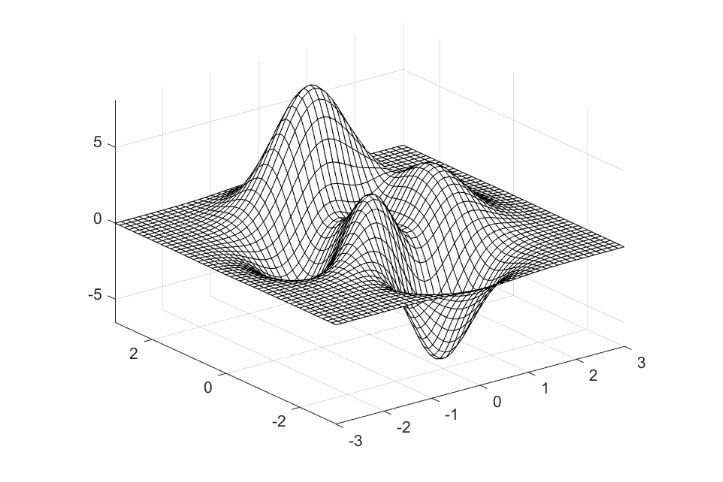
\includegraphics[width=\textwidth,height=\textheight,keepaspectratio]{matlab.png}
  \caption{Visualization of a 3D-mesh in Matlab}
  \label{graphic:mesh-visualization}
\end{figure}

In parallel to MATLAB and R, Python represents the advent of the so-called scripting languages. Scripting languages are programming  languages which offer readability and versatility, along with decoupling from the actual operating system that it is being executed on. System languages, such as C, are designed and used in order to interact directly with the computer hardware, and to constitute data structures from the ground up \citep{ousterhout_scripting_1998}. On the other hand, scripting languages were designed and used in order to connect existing software systems or data sources together, most notably in the early days of shell scripting (such as \lstinline{Bash}, \lstinline{sed} or \lstinline{awk}). Starting with the late 1990s, and the appearance of languages such as Perl\footnote{First version developed in 1987 by Larry Wall} and Python\footnote{First official release in 1991 by Guido Van Rossum}, scripting languages became more widely used by non-programmers who already had data to work with and needed tools to exploit it. In the following decades, the development of additional scientific libraries such as \emph{SciKit}, \emph{NumPy} for mathematics and numerical work or \emph{NLTK} for language processing and social sciences in Python complemented the language's ease of use by providing manipulation of complex scientific concepts \citep{millman_python_2011}, a phenomenon of user-extension which has also been observed in R and MATLAB's ecosystems \citep{moler_history_2020}.

This steady rise of scientific computing has nonetheless highlighted the apparent lack of quality standards in academic software, and how the lack of value judgments on the software written might impact the reliability of the scientific output. Perhaps the most well-known example of such a lack is the one revealed by the leak of the source code of the Climate Research Unit from the University of East Anglia in 2009 \citep{merali_computational_2010}. In the leak, inline comments of the authors, show that particular variable values were chosen to make the simulation run, with scientific accuracy being only a secondary concern. Code reviews of external software developers point out to the code of the CRU leak as being a symptom of the general state of academic software. As Professor Darrel Ince stated to the UK Parliamentary Committee in February 2010:

\begin{quote}
  There is enough evidence for us to regard a lot of scientific software with worry. For example Professor Les Hatton, an international expert in software testing resident in the Universities of Kent and Kingston, carried out an extensive analysis of several million lines of scientific code. He showed that the software had an unacceptably high level of detectable inconsistencies. \citep{committee_disclosure_2010}
\end{quote}

As a response to this realization, the beginning of the 2000s has seen the desire to re-integrate the best practices of software engineering in order to correct scientific software's lack of accuracy \citep{hatton_how_1994}, resulting in the formation of communities such as the Research Software Engineers\citep{woolston_why_2022}. As we have seen above, software engineering had developed on their own since its establishment as an independent discipline and professional field. Such a split, described by Diane Kelly as a "\emph{chasm}" \citep{kelly_software_2007} then had to face the different standards to which commercial software and scientific software were held to. For instance, commercial software must be extensible and performant, two qualities that do not necessarily translate to an academic setting, in which software might be written within a specific, time-constrained, research project, or in which access to computing resources (i.e. supercomputers) might be less of a problem.

Within Landau et. al's conception of the scientific process as the progression from problem to theory, followed by the establishment of a model, the devising of a method, and then on to implemementation and finally to assessment \citep{landau_survey_2011}, code written as academic software is involved in the latter two stages of  method and implementation. Within those two stages, software has to abide by the processes and requirements of scientific research. First and foremost, reproducibility is a core requirement of scientific research in general\footnote{We can date this requirement back to the seventeenth century with Robert Boyle and the Invisible College in England \citep{leveque_reproducible_2012}} and bugs in a scientific software system can lead to radically different ouptuts given slightly different input data, while concealing the origin of this difference. Good academic code, then, is one which defends actively against these, perhaps to the expense of performance and maintainability. This can be addressed by reliable error-handling, regular assertions of the state of the processed data and extensive unit testing \citep{wilson_best_2014}.

Furthermore, a unique aspect of scientific software comes from the lack of clear upfront requirements. Such requirements, in software development, are usually provided ahead of the programming process, and should be as complete as possible. As the activity of scientists is defined by an incomplete understanding of the application domain, requirements tend to emerge as further knowledge is developed and acquired \citep{segal_when_2005}. As a result, efforts have been made to familiarize scientists with software development best practices, so that they can implement quality software on their own. Along with field-specific textbooks\footnote{See \emph{Effective Computation in Physics} \citep{scopatz_effective_2015} or \emph{A Primer for Computational Biology} \citep{oneil_primer_2019} covering similar software-oriented material from different academic perspectives.} the most prominent initiative in the field is \emph{Software Carpentry}, a collection of self-learning and teaching resources which aims at implementing software best practices across academia, for scientists and by scientists. Founded by Greg Wilson, the co-editor of \emph{Beautiful Code}, the organization's title refers directly to equivalents in the field of software development.

We see a convergence of quality standards of broad academic software towards the quality standards of commercial software development\footnote{See Graphbrain at \url{https://github.com/graphbrain/graphbrain} for such an example. The code's organization and formal features are congruent and on par with commercial software.}.  And yet, this convergence is due to, as we have seen, a past divergence between computation and science, as computer science worked towards asserting and pursuing its own field of research. As a subset of science, computer science nonetheless possesses its own specific standards, taking software not as a means to an end, but as the end itself.

\vspace{1\baselineskip}

\subsubsection{Computation as an end}

Computer scientists are scientists whose work focuses on computation as a means, rather than as a tool. They study the phenomenon of computation, investigating its nature and effects through the development of theoretical frameworks around it. Originally derived from computability theory, as a branch of formal mathematical logic, computation emerged as an autonomous field from work in mechanical design and configuration (Ada Lovelace and Charles Babbage),  work on circuit and language design (C. S. Pierce, Konrad Zuse and John Von Neumann), work on mathematical foundations (Alan Turing and Alonzo Church), information theory (Claude Shannon), systems theory (Norbert Wiener) and expert systems (John McCarthy and Marvin Minsky) \citep{ifrah_universal_2001}. In the middle of such a constellation ranging from mathematical theory to practical electronics, computer science establishes its institutional grounding with the inauguration of the first dedicated academic department at Purdue University in 1962.

From this multifaceted heritage and academic interdisciplinarity, computer scientists identified key areas such as data structures, algorithms and language design as foundations of the discipline \citep{wirth_algorithms_1976}. Though the process, the tracing of the "roots" of computation remained a constant debate as to whether computer science exists within the realm of mathematics, of engineering or as a part of the natural sciences. The logico-mathematical model of computer science contends that one can do computer science without an electronic computer, while the engineering approach of computer science tends to put more practical matters, such as architecture, language design and systems programming (implicitly assuming the use of a digital computer) at the core of the discipline; both being a way to generate and process information as natural phenomenon \citep{tedre_development_2006}.

The broad difference we can see between these two conceptions of computer science is that of \emph{episteme} and \emph{techne}. On the theoretical and scientific side, computer science is concerned with the primacy of ideas, rather than of implementation. The quality of a given program is thus deduced from its formal (in the mathematical sense) properties, rather than its formal (in the aesthetic sense) properties. The first manifestations of such a theoretical focus can be found in the Information Processing Language (1956 by Allen Newell, Cliff Shaw and Herbert Simon), which was originally designed and developed to prove Bertrand Russell's \emph{Principia Mathematica}. While the IPL, as one of the very first programming languages, influenced the development of multiple subsequent languages, some later languages came to be known as logic programming languages, based on a formal logic syntax of facts, rules and clauses about a given domain and whose correctness can be easily proven (see \ref{code:prolog_sample} below for an example of the \emph{Prolog} logic programming language).

\begin{listing}
  \inputminted{prolog}{./corpus/inductive.pl}
  \caption{Prolog sample source}
  \label{code:prolog_sample}
\end{listing}

Due to its Turing-completeness, one can write programs such as language processing, web applications, cryptography or database programming (using the \emph{Datalog} variant of \emph{Prolog}), but its use seems to remain limited outside of theoretical circles in 2021\footnote{See the Stackoverflow Developer survey for popular language uses \url{https://insights.stackoverflow.com/survey/2021}}.

Another programming language shares this feature of theoretical soundness faced with a limited range of actual use in production environments, Lisp—\emph{LISt Processor}—designed to process lists. It was developed in 1958, the year of the Dartmouth workshop on Artificial Intelligence, by its organizator, John McCarthy. Inheriting from IPL, it retained the core idea that programs should separate the knowledge of the problem (input data) and ways to solve it (internal rules), assuming  the rules are independent to a specific problem.

The base structural elements of LISP are not symbols, but lists (of symbols, of lists, of nothing), and they themselves act as symbols (e.g. the empty list). By manipulating those lists recursively—that it, processing something in terms of itself—Lisp highlights even further this tendency to separate computation from the problem domain, and to exhibit autotelic tendencies. This is facilitated by its atomistic and relational structure: in order to solve what it has do, it evaluates each symbol and traverses a tree-structure in order to find a terminal symbol. Building on these features of complex structures with simple elements, Willam Byrd, computer scientst at the University of Utah, describes the following lines of Scheme (a LISP dialect) as "the most beautiful program ever written" \citep{byrd_william_2017}, a Scheme interpreter written in Scheme (\ref{code:scheme_interpreter}):

\begin{listing}
  \inputminted{scheme}{./corpus/interpreter.scheme}
  \caption{Scheme interpreter written in Scheme}
  \label{code:scheme_interpreter}
\end{listing}

The beauty of such a program, for Byrd, is the abilty of these fourteen lines to reveal powerful and complex ideas about the nature and process of computation. As an interpreter, this program can take any valid Scheme input and evaluate it correctly, recreating computation in terms of itself. It does so by showing and using ideas of recursion (with calls to \lstinline{eval-expr}), environment (with the evaluation of the \lstinline{body}) and lambda functions, as used throughout the program. Following Alan Kay, creator of the Smalltalk programming language, Byrd equates the feelings he experiences in witnessing and pondering the program above to those suggested by Maxwell's equations, which constitute the foundation of classical electromagnetism (see \ref{graphic:maxwell-equations}) \citep{kay_conversation_2004}. In both cases, the quality ascribed to those inscriptions come from the simplicity and conciseness of their base elements—making it easy to understand what the symbols mean and how we can compute relevant outputs—all the while allowing for complex consequences for both, respectively, computer science and electromagnetism.

\begin{figure}
  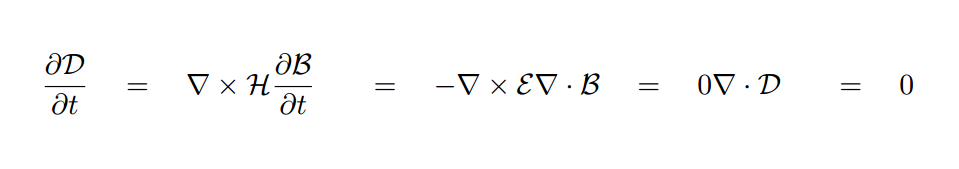
\includegraphics[width=\textwidth,height=\textheight,keepaspectratio]{maxwell.png}
  \caption{Maxwell's equations form a terse, unified basis for electromagnetism, optics and electric circuitry.}
  \label{graphic:maxwell-equations}
\end{figure}

With this direct manipulation of symbolic units upon which logic operations can be performed, Lisp became the language of AI, an intelligence conceived first and foremost as abstractly logical, if not outright algebraic. Lisp-based AI was thus working on what Seymour Papert has called "toy problems"—self-referential theorems, children's stories, or simple puzzles or games \citep{nilsson_early_2009}. In these, the problem and the hardware are reduced from their complexity and multi-consequential relationships to a finite, discreete set of concepts and situations. Confronted to the real world—that is, to commercial exploitation—Lisp's model of symbol manipulation, which proved somewhat successful in those early academic scenarios, started to be applied to issues of natural language understanding and generation in broader applications. Despite disappointing reviews from government reports regarding the effectiveness of these AI techniques, commercial applications flourished, with companies such as Lisp Machines, Inc. and Symbolics offering Lisp-based development and support. Yet, in the 1980s, over-promising and under-delivering of Lisp-based AI applications, which often came from the combinatorial explosion deriving from the list- and tree-based representations, met a dead-end.

\vspace{1\baselineskip}

"\emph{By making concrete what was formerly abstract, the code for our Lisp interpreter gives us a new way of understanding how Lisp works}", notes Michael Nielsen in his analysis of Lisp, pointing at how, across from the \emph{episteme} of computational truths stands the \emph{techne} of implementation \citep{nielsen_lisp_2012}. The alternative to such abstract, high-level language, is then to consider computer science as an engineering discipline, a shift between theoretical programming and practical programming is Edsger Dijkstra's \emph{Notes on Structured Programming}. In it, he points out the limitation of considering programming exclusively as a concrete, bottom-up activity, and the need to formalize it in order to conform to the standards of mathematical logical soundness. Djikstra argues for the superiority of formal methods through the need for a sound theoretical basis when writing software, at a time when the software industry is confronted with its first crisis.

Within the software engineering debates, the theory and practice distinction had a slightly different tone, with terms like “art” and “science” labeling two different mindsets concerning programming \citep{knuth_art_1997}. As mentioned by Djikstra's example, software engineering suffered from an earlier image of programming as an inherently unmanageable, unsystematic, and artistic activity. There again, many saw programming essentially as an art or craft \citep{tedre_development_2006}, rather than an exact science. Beyond theoretical soundness, computer science engineering concerns itself with efficiency and sustainability, with measurements such as the \emph{O()} notation for program execution complexity. It is not so much about whether it is possible to express an algorithm in a programming language, but whether it is possible to run it effectively, in the contingent environments of hardware, humans and problem domains\footnote{Notably, algorithms in textbooks tend to be erroneous when used in production; only in five out of twenty are they correct \citep{pattis_textbook_1988}.}.

This approach, halfway between science and art, is perhaps best seen in Donald Knuth's magnum opus, \emph{The Art of Computer Programming}. In it, Knuth summarizes the findings and achievements of the field of computer science in terms of algorithm design and implementation, in order to "\emph{to organize and summarize what is known about the fast subject of computer methods and to give it firm mathematical and historical foundations.}" \citep{knuth_art_1997}. The art of computer programming, according to him, is therefore based on mathematics, but nonetheless different from it insofar as it does have to deal with effectiveness, implementation and contingency\footnote{\emph{The Art of Computer Programming} involves a hypothetical computer, called MIX, to implement the algorithms discussed.}. In so doing, Knuth takes on a more empirical approach to programming than his contemporaries, inspecting source code and running software to assess their performance, an approach he first inaugurated for FORTRAN programs when reporting on their concrete effectiveness for the United States Department of Defense \citep{defensetechnicalinformationcenter_dtic_1970}.

\emph{Structure and Interpretation of Computer Programs} is another influential academic textbook dealing not just with computation as a an autotelic phenomenon, in which the authors insist that source code is "\emph{must be written for people to read, and only incidentally for machines to execute}" \citep{abelson_structure_1979}. Still, even when confronted with implementation and the plurality of contingencies of non-mathematical elements which accompanies it, the aesthetic standard in this more engineering approach to computer science is the proportionality between the number of lines of code written and the complexity of the idea explained, as we can see in the series \emph{Beautiful Julia Algorithms} \citep{moss_beautifulalgorithms_2022}. For instance, \ref{code:bubble_sort_julia} implements the Bubble Sort sorting algorithm in one loop rather than the usual two loops in C, resulting in an easier grasping of the concept at hand, rather than being distracted by the idiosyncracy of the implementation. The simplicity of scientific algorithms is expressed even further in \ref{code:nearest_neighbor_julia} the one-line implementation of a procedure for finding a given element's nearest neighbor, a crucial component of classification systems, including AI systems.

\begin{listing}
  \inputminted{julia}{./corpus/bubblesort.jl}
  \caption{Bubble Sort implementation in Julia}
  \label{code:bubble_sort_julia}
\end{listing}

\begin{listing}
  \inputminted{julia}{./corpus/nearest_neighbor.jl}
  \caption{Nearest neighbor implementation in Julia}
  \label{code:nearest_neighbor_julia}
\end{listing}

According to Tedre, computer science itself was split in a struggle between correctness and productivity, between theory and implementation, and between formal provability and intuitive art \citep{tedre_science_2014}. In the early developments of the field, when machine time was expensive and every instruction cycle counted, efficiency ruled over elegance, but in the end he assesses elegance prevailed, as we will see with the evolution of craft within programming in section \ref{sec:craft} below.

In closing, one should note that the \emph{Art} in the title of Knuth's series does not, however, refer to art as a fine art, or a purely aesthetic object. In a 1974 talk at the ACM, Knuth goes back to its Latin roots, where we find \emph{ars}, \emph{artis} meaning "skill.", noting that the equivalent in Greek being τεχνη, the root of both "technology" and "technique.". This semantic proximity helps him reconcile computation as both a science and an art, the first due to its roots in mathematics and logic, and the second

\begin{quote}
  because it applies accumulated knowledge to the world, because it requires skill and ingenuity, and especially because it produces objects of beauty. A programmer who subconsciously views himself as an artist will enjoy what he does and will do it better. Therefore we can be glad that people who lecture at computer conferences speak about the state of the Art. \citep{knuth_computer_1974}
\end{quote}

\vspace{1\baselineskip}

When written within an academic and scientific context, source code tends to align with the aesthetic standards of software development, valuing reliability, reabability, sustainability, in particular through Greg Wilson's work on the development of software development principles through the Software Carpentry initiative. This alignment can also be seen in a conception of computer science as a kind of engineering, as an empirical practice which can and should still be formalized in order to become more efficient. There, one can turn to Donald Knuth's \emph{Art of Computer Programming} to see the connections between the academia's standards and the industry's standards.

And yet, a conception of computation as engineering isn't the only conception of computer science. Within a consideration of computer science as a  theoretical and abstract object of study, source code becomes a means of providing insights into more complex abstract concepts, seen in the Lisp interpreter, or one-line algorithms implementing foundational algorithms in computer science, similar to this aspect of the hacker ethos. It is this relation to a conception of beauty traditionally associated with mathematics and engineering which we will investigate further to highlight which aesthetic ideals can be ascribed to code. But, first, we complete our overview of code practitioners by turning to the software artists, who engage most directly with source code as a written material through source code poetry.

\pagebreak

\subsection{Poets}
\label{subsec:poets}

Source code poetry is a distinct subset of electronic literature, and software art. One the one hand, electronic literature is a broad field encompassing natural language texts taking full advantage of the dynamic feature of computing to redefine the concept of text, authorship and readership. It encompasses a variety of approaches, including generative literature, interactive fiction, visual poetry, source code poetry and esoteric programming languages, as well as certain aspects of software art. However, we focus here only on the elements of electronic literature which shift their focus from output to input, from executable binary with transformed natural language as a result, to static, latent source.

On the other hand, software art is an umbrella term regrouping artistic practices which engage with the computer on a somewhat direct, material level, whether through hardware\footnote{See Alexei Shuglin's \emph{386 DX} (1998-2013)} or software\footnote{See Netochka Nezanova's \emph{Nebula.M81} (1999)}. This space for artistic experimentation flourished at the dawn of the 20th century, with initiatives such as the \emph{Transmediale} festival's' introduction of a \emph{software art} award between 2001 and 2004, or the \emph{Run\_me} festival, from 2002 to 2004. In both of these, the focus is on projects which incorporate standalone programmes or script-based applications which aren not merely functional tools, but also act as an effective artistic proposition, as decided by the artist, jury and public. These works often bring the normally hidden, basic materials from which digital works are made (e.g. code, circuits and data structures) into the foreground \citep{yuill_code_2004}. Within this realm, code poetry is a form a software art whose execution is only secondary to the work's meaning.

Electronic literature, a form based on the playful \emph{détournement} of the computer's constraints, gets closer to our topic insofar as the poems generated represent a more direct application of the rule-based paradigm to the syntactical output of the program. Starting with Christopher Stratchey's love letters (1953), generated (and signed!) by MUC, the Manchester Univac Computer, computer poems are generated by algorithmic processes, and as such rely essentially on this particular feature of programming: laying out rules in order to synthesize syntactically and semantically sound natural language poems. Here, the rules themselves matter only in relation to the output, as seen by their ratio: a single rule for a seemingly-infinite amount of outputs, with these outputs very often being the only aspect of the piece shown to the public.

These works and their authors build on a longer tradition of rule-based composition, from Hebrew to the Oulipo and John Cage's indeterministic composition, amongst others \citep{cramer_words_2003}, a tradition in which creativity and beauty can emerge from within a strict framework of formal rules. Nonetheless, the source code to these works is rarely released in conjunction with their output, hinting again at their lesser importance in terms of their overall artistic values. If electronic literature is composed of two texts, a natural-language output and a computer-language source, only the former is actually considered to be poetry, often leaving the latter in its shadow (as well as, sometimes, its programmer, an individual sometimes different from the poet). The poem exists through the code, but isn't exclusively limited to the human-readable version of the code, as it only comes to life and can be fully appreciated, under the poet's terms, once interpreted or compiled. While much has been written on electronic literature, few of those commentaries focus on the soundness and the beauty of the source as an essential component of the work, and only in recent times have we seen the emergence of close-readings of the source of some of these works for their own sake\footnote{See the publications in the field of Critical Code studies, Software studies and Platform studies.}. These constitute a body of work centered around the concept of generative aesthetics \citep{goriunova_read_2005}, in which beauty comes from the unpredictable and somewhat complex interplay of rule-based systems, and whose manifestations encompass not only written works, but games, visual and musical works as well.

And yet, the approach of code poets is more specific than broad generative aesthetics: it is a matter of exploring the specific expressive affordances of source code, and the overlap of machine-meaning and human-meaning essential to the correct functioning of code which acts as a vector for artistic communication. Such an overlap of meaning is a specific feature of source code poetry. In a broad sense, code poetry conflates classical poetry (as strict syntactical and phonetical form, combined with poetic expressivity) with computer code, but it is primarily defined by the fact that it does not require the code to be executed, but only to be read by a human. Following the threads laid out by electronic literature, code poetry starts from this essential feature of computers of working with strictly defined formal rules, but departs from it in terms of utility. Code poems are only functional insofar as they are accepted by the intepreter or compiler of the language in which they are written. To the computer, they are indeed functional, in that they are legal and can be parsed; but they do not do anything of \emph{use}. Such formal compliance is only a pre-requisite, a creative constraint, for their human writers.

Within this reliance on creative constraints provided by a computing environment, the emphasis here is on the act of reading, rather than on the act of deciphering, as we have seen with obfuscated code (and in functional code in general). Source code poems are often easy to read, and have an expressive power which operates beyond the common use of programming. Building on Flusser's approach, let us consider poetry as a means to bring concepts into the thinkable, and to crystallize thoughts which are not immediately available to us \citep{flusser_doubt_2014}; through various linguistic techniques, poetry allows us to formulate new concepts and ideas, and to shift perspectives.

In their different manifestations, code poems make the boundary between computer meaning and human meaning thinner and thinner, a feature often afforded by the existence and use of higher-level programming languages. Starting with the development of FLOWMATIC in 1955 by Grace Hopper, it was shown that an English-like syntactical system could be used to communicate concepts for the computer to process. From there, programming languages could be described along a gradient, with binary at the lowest end, and natural language (in an overwheling majority, English) at the highest end. This implies that they could be written and read similarly to English, including word order, pronouncation and interpretation, similar to the error-tolerance of human laguages, which doesn't cause the whole communication process to fail whenever a specific word, or a word order isn't understood.

The community of programmers writing in Perl, \emph{perlmonks}\footnote{See their website: \url{https://perlmonks.org/}, with the spiritual, devoted and communal undertones that such a name implies.} has been one of the most vibrant and productive communities when it comes to code poetry. This particular use of Perl started in 1990, when the language creator Larry Wall shared some of the poems written in the language, and it gained further exposition through the work of Shannon Hopkins \citep{hopkins_camels_1992}. The first Perl poem is considered to have been written by Wall in 1990, reproduced in \ref{code:japh_perl}.

\begin{listing}
  \inputminted{perl}{./corpus/japh.pl}
  \caption{Just Another Perl Hacker, japh.pl}
  \label{code:japh_perl}
\end{listing}

Hopkins analyzes the ability of the poem to enable dual understandings of the source—human and machine. Yet, departing from the previous conceptions of source that we have looked at, code poetry does not aim at expressing the same thing to the machine and to the human. The value of a good poem comes from its ability to evoke different concepts for both readers of the source code. As Hopkins puts it:

\begin{quote}
  In this poem, the q operator causes the next character (in this case a newline) to be taken as a single quote, with the next occurrence of that delimiter taken as the closing quote. Thus, the single-quoted line 'Just another Perl hacker' is printed to STDOUT. In Perl, the "unless \$spring" line is mostly filler, since \$spring is undefined. In poetical terms, however, "\$spring" is very important: haiku poetry is supposed to specify (directly or indirectly) the season of the year. As for the q operator, that reads in English as the word "queue", which makes perfect sense in the context of the poem. \citep{hopkins_camels_1992}
\end{quote}

The poem \emph{Black Perl} in \ref{code:black_perl}, submitted anonymously, is another example of the richness of the productions of this community:


\begin{listing}
  \inputminted{perl}{./corpus/black_perl.pl}
  \caption{lBlack Perl, Anonymous, 1990, updated by kck, 2017}
  \label{code:black_perl}
\end{listing}

The most obvious feature of this code poem is that it can be read by anyone, including by readers with no previous programming experience: each word is valid both as English and as Perl. A second feature is the abundant use of verbs. Perl belongs to a family of programming languages grouped under the \emph{imperative} paradigm, which matches a grammatical mood of natural languages, the \emph{imperative mood}. Such mood emphasizes actions to be take rather than, for instance, descriptions of situations, and thus sets a clear tone for the poem. The fact that Perl is based on stating procedures to be executed and states to be changed creates this feeling of relentless urgency when reading through the poem, a constant need to be taking actions, for things to be changed. Here, the native constraints of the programming language interacts directly with the poetic suggestion of the work in a first way: the nature of Perl is that of giving orders, resulting in a poem which addresses \emph{someone} to execute \emph{something}. Still, Perl's flexibility leaves us wondering as to who and what are concerned by these orders. Is the poem directing its words to itself? To the reader? Is Perl just ever talking exclusively to the computer? This ambiguity of the adressee adds to the ominousness of each verse.

Following in the footsteps of the \emph{perlmonks}, additional communities around code poetry have formed, whether in university settings\footnote{Such as Stanford's Code Poetry Slam, which ran between 2014 and 2016, see \url{https://web.archive.org/web/20161024152353/http://stanford.edu/\%7Emkagen/codepoetryslam/} }, or as independent intiatives\footnote{See the Source Code Poetry event, \url{https://www.sourcecodepoetry.com/}}. Beyond collections such as threads and hashtags on Twitter\footnote{See \lstinline{#SongsInCode} at \url{https://twitter.com/search?q=\%2523SongsInCode}}, code poetry also features artistic publications, such as printed anthologies of code poetry in book form \citep{bertram_code_2012} \citep{holden_code_2016}.

Yet, code poems from the 20th century aren't the first time where a part of the source code is written exclusively to elicit a human reaction, without any machinic side-effects. One of the earliest of those instances is perhaps the Apollo 11 Guidance Computer (AGC) code, written in 1969\footnote{Hamilton et. al., 1969, retrieved from https://github.com/chrislgarry/Apollo-11} in Assembly. Cultural references and jokes are peppered throughout the text as comments, asserting computer code as a means of expression beyond exclusively technical tasks\footnote{See also: "Crank that wheel", "Burn Baby Burn"}, and independent from a single writer's preferences, since they passed multiple checks and review processes to end up in the final, submitted and executed document, such as reproduced in \ref{code:numero_mysterioso_asm}.

\begin{listing}
  \inputminted{ca65}{./corpus/numero_mysterioso.asm}
  \caption{AGC source code for the Lunar Landing Guidance Equation, 1969}
  \label{code:numero_mysterioso_asm}
\end{listing}

Code comments allow a programmer to write in their mother tongue, rather than in the computer's, enabling more syntactic and semantic flexibility, and thus reveal a burgeoning desire for programmers to express themselves within their medium of choice.

At the turn of the 1980s, following the transition to programming from an annex practice to full-fledged discipline and profession, and with the development of more expressive programming languages (e.g. Pascal in 1970, C in 1972), software development had grown exponentially\footnote{See Stackoverflow's Developer Profile survey: \url{https://insights.stackoverflow.com/survey/2019\#developer-profile-_-years-since-learning-to-code}}, and fostering practices, communities and development styles and patterns\footnote{From Djikstra's Notes on Structured Programming to Knuth's Literate Programming and Martin's Clean Code}. Source code becomes recognized as a text in its own, which can hold qualities and defects of its own, and to which engineering and artistic attention must be paid. No longer a transitional state from formula to binary, it becomes a semantic material, whose layout, organization and syntax are important to the eyes of its writers and readers. Pushing further into the direction of the visual layout of the code, such an endeavour becomes pursued for its own sake, equally important to the need for a program to be functional.

The Obfuscated C Code Contest\footnote{\url{https://www.ioccc.org}}, starting in 1984, is the most popular and oldest organized production of such code, in which programmers submit code that is functional and visually meaningful beyond the exclusive standards of well-formatted code. If the source code's two meanings of a computer poem was made readily available to interpretation, and if such meanings existed in parallel in the comments of the AGC routines, pointing at the overlay of computer-related semantics (e.g. line numbers) and human-related semantics (e.g. a reference to the biblical number of the beast, 666), obfuscated code is a first foray into closely intertwining these separate meanings in the source code itself, making completely transparent, or completely opaque what the code does just by glancing at it.

\begin{listing}
  \inputminted{c}{./corpus/circle.c}
  \caption{westley.c, entry to the 1988 IOCCC}
  \label{code:circle_c}
\end{listing}

The source code in \ref{code:circle_c}, submitted to the 1988 IOCCC\footnote{Source: \url{https://web.archive.org/web/20131022114748/http://www0.us.ioccc.org/1988/westley.c}} is a procedure which does exactly what it shows: it deals with a circle. More precisely, it estimates the value of PI by computing its own circumference. While the process is far from being straightforward, relying mainly on bitwise arithmetic operations and a convoluted preprocessor definition, the result is nonetheless very intuitive—the same way that PI is intuitively related to PI. The layout of the code, carefully crafted by introducing whitespace at the necessary locations, doesn't follow any programming practice of indentation, and would probably be useless in any other context, but nonetheless represents another aspect of the \emph{concept} behind the procedure described, not relying on traditional programming syntax\footnote{For such a program, see for instance: \url{https://crypto.stanford.edu/pbc/notes/pi/code.html}}, but rather on an intuitive, human-specific understanding\footnote{Concrete poetry also makes such a use of visual cues in traditional literary works.}.

Obfuscating practices, beyond their technical necessities (for security and efficiency), are traditionally tied to hacking practices, prominently with one-liners (the shorter a name, the more obscure and general it becomes). As such, they rely on the brain-teasing process of deciphering, and on the pleasurable, aesthetic experience of resolving and uniting two parallel meanings: what we see in the code, and what it does\footnote{Also known informally as the "Aha!" moment, crucial in puzzle design.}. What we focus on here is the aspect of obfuscation which plays with the different layers of meaning: meaning to the computer, meaning to the human, and different ways of representing and communicating this meaning (from uglifying, to consistent formatting, to depicting a circle with dashes and underscores). While the aesthetics at play in hacking will be further explored below, we focus on the fact that obfuscating code practices, beyond hiding the meaning and the intent of the program, also manifest an attempt to represent such a meaning in different ways, leaving aside traditional code-writing practices and suggesting the meaning of the program by challenging the abilities of human interpretation at play in the process of deciphering programs.

Code poetry values code which, while being functional, expresses more than what it does, by allowing for \emph{Sprachspiele}, languages games where pronounciation, syntax and semantics are playfully composed into a fluid linguistic construct in order to match a human poetic form, such as the haiku, or to constitute a specific puzzle. Relying on the inherent tendency of source code to remain opaque, obfuscated code contests let us see how far can such an opacity of a computer program's effective meaning be sustained.

\vspace{1\baselineskip}

In this section, we have seen how the set of individuals who write and read code is heterogeneous. Instead, we can see a significant degree of variation between source code written within the context of software engineering, hacking, scientific research and artistic activity. While none of these areas are exclusive of the others—a software developer by day can hack on the weekend and participate in code poetry events—, they do convey different perspectives on how the code is written, and on how it is evaluated. This cursory introduction to each approach has shown that, for instance, software engineers prefer code which is modular, modifiable, sustainable and understandable by the largest audience of possible contributors, while hackers would favor conciseness over expressivity, and tolerate idiosyncracy for the purpose of immediate, functional efficiency. On the other hand, scientific programming favors ease of use, accuracy and reproducibility, sometimes overlapping with software engineering, while code poets explore the semantic tension between a human interpretation and the machine interpretation of a given source code.

These are strands of similarity within apparent diversity. The code snippets in this section show that there is a tendency to prefer a specific group of qualities—readability, conciseness, clarity, expressivity and functionality—even though different types of the aforementionned practices would put a different emphasis on each of those aspects. The question we turn to next, then, is to what extent do these different practices of code writing and reading share common judgments regarding their formal properties? Do hackers and poets agree on some value judgment, and how? To start this investigation, we first analyze programmers' discourses in the following section in order to identify concrete categories of formal properties which might enable a source code to be positively valued for its appearance, before we turn to the aesthetic registers code practicionners refer to when discussing beautiful code to further qualifies these properties.

\pagebreak

\section{Ideals of beauty}

With this overview of the varieties of practices at play amongst those who read and write source code, we will analyze more thoroughly what are the aesthetic standards most value by those different groups. The aim here is to formalize our understanding of which source code is considered beautiful, and to do so at multiple levels. The goal here is to capture both the specific manifestations of beautiful code as specified and enunciated by programmers, as well as the semantic contexts from which these enunciations originate. What we will see is that, while a set of aesthetic values and a set of aesthetic manifestations can be pinpointed precisely, the domains that are mobilized to justify these values are clearly distinct. To do so, we will introduce a discourse analysis framework for the empirical study of the corpus, followed by an examination of the broad fields that these discourses refer to. This will be complemented in Chapter 3 by a a medium-specific reading through critical code studies and rhetorical code studies on one hand, and the work done by conceptual metaphors on the other.

\subsection{Introduction to the Methodology}

Discourse consists of text, talk and media, which express ways of knowing the world, of experiencing and valuing the world. This study builds on Kintsch and Van Dijk's work on providing tools to analyze an instance of discourse, and is centered around what is said to constitute good source code. While discourse analysis can also be used critically by unearthing which value judgments that occur in power relationships\footnote{See Diana Mullet on Critical Discourse Analysis \citep{mullet_general_2018a}}, we focus here on aesthetic value judgments, as their are first expressed through language. Of all the different approaches to discourse, the one we focus on here is that of \emph{pragmatics}, involving the spatio-temporal and intentional context in which the discourse is uttered. We find this approach particularly fitting through its implication of the \emph{cooperative principle}, in which utterances are ultimately related to one another through communicative cooperation to reveal the intent of the speaker \citep{schiffrin_approaches_1994}. Practically, this means that we assume the position of programmers talking to programmers is cooperative insofar as both speaker and listener want to achieve a similar goal: writing good code. This double understanding—focusing first and foremost on utterances, and then re-examining them within a broader cooperative context—will lead us to encompass a variety of production media (blog post, forums, conferences, text books), in order to depict the cultural background (software practices as outlined above as well as additional factors such as skill levels). Our comprehension of those texts, then, will be set in motion by a a dual movement between local, micro-units of meaning and broader, theoretical macro-structure of the text, and linked by acts of co-reference \citep{kintsch_model_1978}.

Particular attention will be paid to the difference between intentional and extensional meaning \citep{dijk_strategies_1983}. As we will see, some of the texts in our corpus tend to address a particular problem (e.g. on forums, social media or question \& answer platforms), or to discuss broader concepts around well-written code. Particularly,

\begin{quote}
  Figures of speech may attract attention to important concepts, provide more cues for local and global coherence, suggest plausible pragmatic interpretations (e.g., a promise versus a threat), and will in general assign more structure to elements of the semantic representation, so that [meaning] retrieval is easier. \citep{dijk_strategies_1983}
\end{quote}

Following this idea, we will proceed by examining syntactic markers to deduce overarching concepts at the semantic level. Among those syntactic markers, we include single propositions as explicit predicates regarding source code, lexical fields used in those predicates in order to identify their connotations and denotations, as well as for the tone of the enunciations to identify value judgments. At the semantic level, we will examine the socio-cultural references, the \emph{a priori} knowledge assumed from the audience, as well as the semantic entities which compose the theme of the discourse at hand. Finally, the discourses we will examine aren't exclusively composed of natural language, but also of source code extracts, resulting in a hybrid between natural and machine syntax within the same discursive artifact.

In line with John Cayley's analytic framework of structure, syntax and vocabulary \citep{cayley_code_2012}, we can nonetheless echo discourse analysis as applied to natural languages. Cayley's framework highlights essential aspect of analysis which applies both to natural languages and source code: that of the scales at which aesthetic judgment operates. It also provides a bridge with literature and literary studies without imposing too rigid of a grid preventing interdisciplinarity. While it does not immediately acknowledge more traditional literary concepts such as fiction, authorship, literarity, etc., Cayley's framework does leave room for these concepts to be taken into account. Particularly, we will see that the concept of authorship—who writes to whom—will prove to be useful.

Finally, our intepretation of the macrostructures described by Kintsch and Van Dijk will rely extensively on the work done by metaphors as the conceputal level, rather than at the strictly linguistic one. Lakoff and Johsnon's seminal work develops a theory of conceptual metaphors by highlighting their essential dependence on pre-existing cognitive structures, which we associate with already-understood concepts. The metaphor maps a source domain (made up of cognitive structure(s)) to a target domain. In the process, they extend the field of applicability of metaphors from the strictly literary to the broadly cultural: metaphors work because each of us has some conception of those domains involved in the metaphorical process. Metaphors rely in part on a static understanding, resulting in a fixed meaning from the application of a given source to a given target. Some of these sources are called \emph{schemas}, and are defined enough to not be mistaken for something else, but broad enough to allow for multiple variants of itself to be applied to various targets \citep{lakoff_metaphors_1980}, providing both diversity and reliability. As we will see below, their approach allows us to focus not just on textual objects, but on the vast range of metaphors used specifically in computing-related environments. Given that the source of the metaphor should be grounded, with as little invariablity as possible, in order to qualify a potentially ill-defined target domain, this provides us with a first foray into the inherent elusiveness and instability of computing when presented to a broader audience.

Going beyond the role of metaphors manifested in expressions such as \emph{the desktop}, \emph{the mouse}, or \emph{the cloud}, we will explore Lakoff's understanding of the specifically poetic metaphor in Chapter 3 while assessing the linguistic component of computing—source code. For now, we will pay close attention to what programmers are saying about (beautiful) source code, which metaphors they employ to support these value judgments, and why—focusing first on the metaphors \emph{of} source code, before moving, in the next section, to the metaphors \emph{in} source code.

The corpus studied here consists of texts ranging from textbooks and trade manuals to blog posts and online forum discussions\footnote{Specifically, we have gathered 47 different online sources, from forum discussions to blog posts, 26 journal articles from the Association for Computing Machinery, 20 monographs and 1 edited volume, listed in Appendix I. These constitute our primary sources insofar as they are written by practicioners on the topic of good and beautiful code.}. The rationale behind such a broad approach is to constitute a lexical basis for what practicing programmers consider when assessing good code, as expressed in the everyday interactions of online forums and blog posts, but also inclusive of diverse sources of communication, beyond edited volumes. From authoritative sources, such as canonical textbooks or widely-read blog posts from well-known practicioners, to more casual forum exchanges will support the empirical dimension of our research. From this approach, this section will show how there are \emph{specific} ways to qualify well-written code, which are echoed both from bottom-up and from top-down perspectives, and employing recurring references.

\subsection{Lexical Field in Programmer Discourse}

In terms of existing studies of the lexical field programmers use, Erik Pineiro has done significant work in his doctoral thesis. In it, he argues that aesthetics exist from a programmers perspective, decoupled from the final, executable form of the software. While this current study draws on his work, and confirms his findings, it also builds upon it in several ways. First, Pineiro focuses on a narrower corpus, that of the Slashdot.org\footnote{\url{https://slashdot.org}} forums \citep{pineiro_aesthetics_2003} (p. 51). Second, he examines aesthetic judgment from a private perspective of software engineers, separate from other possible aesthetic fields which might enter in dialogue with beautiful code \citep{pineiro_aesthetics_2003} (p.52), such as artists or hackers. Finally, his discussion of aesthetics takes place in a broader context of business management and productivity, while this current study situates itself within media studies and aesthetic philosphy, and its implications within how a certain class of communicative artefacts are considered beautiful. Still, Pineiro's work provides valuable insights in terms of identifying the manifestations and rationales for an aesthetic experience of source code. Thus, we continue his research by highlighting the main adjectives in the lexical field of programmers' discourse.

\vspace{1\baselineskip}

Already mentioned in Peter Naur's analysis of the practice of programming, \emph{clean} is the first adjective which stands out as a requirement when assessing the form taken by source code. Clean code, he says, is a reference to how easy it is for readers of code to build a coherent theory of the system both described and prescribed by this source code \citep{naur_programming_1985}. This purpose of cleanliness is then completed by a description of the clean form in an analysis of clean code appears a couple of decades later in the title of a series of best-selling trade manuals written by Robert C. Martin and published by Prentice Hall from 2009 to 2021, the full titles of which clearly enunciate their normative aim\footnote{\emph{Clean Code: A Handbook of Agile Software Craftsmanship}, \emph{The Clean Coder: A Code Of Conduct For Professional Programmers}, \emph{Clean Architecture: A Craftsman's Guide to Software Structure and Design}, \emph{Clean Agile: Back to Basics}, \emph{Clean Craftsmanship: Disciplines, Standards, and Ethics}.}. What exactly is cleanliness, in Martin's terms, is nonetheless defined by circumlocutions, relying on contributions from experts. After asking leading programmers what clean code means to them, he carries on in the volume by providing examples of \emph{how} to achieve clean code, while only loosely defining what it is. In general, cleanliness is mostly a definition by negation: it states that something is clean if it is free from impurities, blemish, error, etc. An alternative to this definition which trade manuals such as \emph{Clean Code} use consists in providing examples on how to move from bad, "dirty" code, to clean code through specific, practical guidelines regarding naming, spacing, class delimitation, etc.. Starting at a high-level, some hints can be glimpsed from Ward Cunningham's answer:

\begin{quote}
  You know you are working on clean code when each routine you read turns out to be pretty much what you expected. You can call it beautiful code when the code also makes it look like the language was made for the problem. \citep{martin_clean_2008} (p.10)
\end{quote}

along with Grady Brooch's:

\begin{quote}
  Clean code is simple and direct. Clean code reads like well-written prose. Clean code never obscures the designer’s intent but rather is full of crisp abstractions and straightforward lines of control. \citep{martin_clean_2008} (p.11)
\end{quote}

Cleanliness is tied to expressiveness: it is devoid of any extraneous syntactic and semantic symbols (e.g. it does one thing, and one thing well), in order to let the problem at hand appear, with all its implications. Instead, the tool (i.e. programming languages) disappear at the syntactic level, to enable expressiveness at the semantic level.

Martin echoes Hunt when he advocates for such a definition of clean as lack of additional syntactic information:

\begin{quote}
  Don't spoil a perfectly good program by over-embellishment and over-refinement. \citep{hunt_pragmatic_1999}
\end{quote}

This advice to programmers denotes a conception of clean that is not just about removing as much syntactic form as possible, but which also implies a balance. \emph{Overembellishment} implies excess addition, while \emph{over-refinement} implies, on the contrary, excess removal. This normative approach finds its echo in the numerous quotations of Antoine de Saint-Exupéry's comment on aircraft design\footnote{For instance, see \url{https://news.ycombinator.com/item?id=1640594} and \url{https://twitter.com/codewisdom/status/1353651398337044481}}:

\begin{quote}
  Il semble que la perfection soit atteinte non quand il n'y a plus rien à ajouter, mais quand il n'y a plus rien à retrancher.  \citep{desaint-exupery_terre_1972}\footnote{\emph{ In anything at all, perfection is finally attained not when there is no longer anything to add, but when there is no longer anything to take away, when a body has been stripped down to its nakedness.}, translated by Lewis Galantière in the 1939 edition of \emph{Wind, Sand and Stars}}
\end{quote}

This balance between too much and too little is found in another dichotomy stated by programmers: between simple and clever. Simplicity, argues Jeremy Gibbons, is not only a restraint on the quantity of syntactic tokens (as one could achieve by keeping names short, or aligning indentations), but also a semantic equilibrium at the level of abstracted ideas \citep{gibbons_beauty_2012}. The balance between breadth and depth regarding the task of the code, between the precision of a use-case and its generalization, and its leveraging of external—i.e. supposedly reliable—code is summed up his quoting of Ralph Waldo Emerson at the conclusion of his column:

\begin{quote}
  We ascribe beauty to that which is simple; which has no superfluous parts; which exactly answers its end; which stands related to all things; which is the mean of many extremes. \citep{gibbons_beauty_2012}
\end{quote}

In another ACM publication, Kristiina Karvonen argues for simplicity not just as a design goal, as leveraged by human-computer interface designers, but as a term with a longer history within the tradition of aesthetic philosophy, especially the work of Johann Joachim Winckelmann \citep{karvonen_beauty_2000}. In particular, she stresses the difficulty "to create significant, that is, beautiful works of art with simple means" \citep{karvonen_beauty_2000}. Here, her correlation between \emph{significance} and \emph{pleasant appearance} hints at the semantic role of simplicity, as a means to communicate ideas (i.e. to \emph{signify}) to an audience.

Precisely, simplicity is correlated with clarity (of meaning); if the former refers mainly to the syntactic component (fewer tokens), it enables the non-obfuscated framing of the ideas at play. One example is given in \ref{code:clearer_method_c} by Dave Bush in a post titled  \emph{15 Ways to Write Beautiful Code}.

\begin{listing}
  \inputminted{c}{./corpus/clearer_method.c}
  \caption{Example of clarity differences between two methods.}
  \label{code:clearer_method_c}
\end{listing}

Here, the strive for simplicity leads to removing the brackets, and flipping the boolean check in the if-statement to add a \lstinline{return}. Even though it is, strictly speaking, more characters than the brackets and newline (six characters compared to four), the program becomes cleaner, and thus clearer, he argues, by separating the two branching cases inherent to the use of conditional logic, under the form of an if-statement. In the second version, it is made clear that, if a condition \emph{is}, the execution should stop, and any subsequent statement can entirely disregard the existence of the if-statement; in the first version, the condition that \emph{is not} is entangled with code that should be executed, since the existence of the if-statement has to be kept in mind until the closing bracket \citep{bush_15_2015}.

As a corollary to clarity stands obfuscation. It is the act, either intentional or un-intentional, to complicate the understanding of what a program does by leading the reader astray through a combination of syntactic techniques, a process we have already seen in the works of the IOCCC above. In its most widely applied sense, obfuscation is used for practical production purposes: reducing the size of code, and preventing the leak of proprietary information regarding how a system behaves. For instance, the JavaScript source code in \ref{code:home_js} is obfuscated through a process called \emph{minification} into the source code in \ref{code:home_minified_js}

\begin{listing}
  \inputminted{js}{./corpus/home.js}
  \caption{home.js (before minification)}
  \label{code:home_js}
\end{listing}

\begin{listing}
  \inputminted{js}{./corpus/home_minified.js}
  \caption{home.js (after minification)}
  \label{code:home_minified_js}
\end{listing}

This process of obfuscation has very clear, quantitative assessment criterias, such as the size of the source code file and cryptographic complexity \citep{pellet-mary_co6gc_2020}. Nonetheless. obfuscation can also be valued as a positive aesthetic standard, of which the IOCCC is the most institutionalized guarantor. These kinds of obfuscations, as Mateas and Montfort analyze, involve the playful exploration of the intertwinings of syntax and semantics, seeing how much one can bend the former without affecting the latter. These textual manipulations, they argue, possess an inherently literary quality:

\begin{quote}
  Obfuscation and weird languages invite us to join programming contexts to the literary contexts that must obviously be considered when evaluating literary code. They also suggest that coding can resist clarity and elegance to strive instead for complexity, can make the familiar unfamiliar, and can wrestle with the language in which it is written, just as much contemporary literature does. \citep{mateas_box_2005}
\end{quote}

Such literary connection can also be seen in Noël Arnaud's work \emph{Poèmes Algol} \citep{arnaud_poemes_1968}, in which he uses the constructs of the language Algol 68 in order to evoke in the reader something different than what the program actually does (i.e. fail to execute anything meaningful). Here, obfuscation is can be considered a literary value, as opposed to other domains, such as the scientific or the architectural, where it is both considered exclusively negatively.

Another insight on simplicity and programming regarding the communication of ideas is hinted at by Richard P. Gabriel in his use of the concept of \emph{compression} in both poetry and programming, there is a desire to increase the semantic charge (or significance, in Karvonen's terms) all the while reducing the syntactic load (or the quantitity of formal tokens). One of those extraneous loads is explanation, as pointed out online by user Mason Wheeler:

\begin{quote}
  When it requires a lot of explanation like that, it's not "beautiful code," but "a clever hack." \citep{stackoverflow_how_2013}
\end{quote}

This answer, posted on the software engineering \emph{Stack Exchange} forum, in response to the question "How can you explain "beautiful code" to a non-programmer?" \citep{stackoverflow_how_2013}, not only highlights the need to be self-explanatory, but also points at a quality departing form simplicity—cleverness.

Cleverness is often found, and sometimes derided, in examples of code written by hackers, since it unsettles this balance between precision and generality. Clever code would tend towards exploiting particularities of knowledge of the medium (the code) rather than the goal (the problem). Hillel Wayne presents the snippet of Python code in \ref{code:is_unique_python} as an example of bad clever code:

\begin{listing}
  \inputminted{python}{./corpus/unique.py}
  \caption{Method to check for the uniqueness of array elements}
  \label{code:is_unique_python}
\end{listing}

Here, the knowledge of how the \lstinline{set()} function in Python behaves, is required in order to understand that the \lstinline{is_unique()} function returns whether all the elements of the given list are unique. A programmer without familiarity with Python would be unable to do so without consulting the Python documentation (i.e. requiring extraneous explanation).

Hillel elaborates on the difference between "bad" clever code\footnote{See, for instance, Duff's device, an idiosyncratic and language-specific way to speed up loop unrolling in C. The author himself feels "a combination of pride and revulsion at this discovery" \citep{duff_tom_1983}}, which is essentiall read-only due to its idiosyncracy and reliance on tacit knowledge, and "good" clever code, and such distinction corroborates our previous observations regarding beautiful code as a means for expression of the problem domain. His example is that the problem of sorting the roughly 300 million U.S. american citizens by birthdate can be made considerably more efficient by cleverly considering that no U.S. american citizen is older than 120 years, whereby radically reducing the computation space.

Meanwhile, cleverness is a valued attribute in the context of hacker code, putting more emphasis on the technical solution than on the problem domain, as we have seen above. A salient is example was the 1994 \lstinline{smr.c} entry to the IOCCC, which aimed at being the smallest self-reproducing program \citep{kanakarakis_international_2022}. An exact reproduction of the source code can be found in \ref{code:smr_c}

\begin{listing}
\inputminted{c}{./corpus/smr.c}
  \caption{smr.c}
  \label{code:smr_c}
\end{listing}

Consisting of a file weighing zero bytes, \lstinline{smr.c} provides both a clever reduction of the problem domain, and a clever understanding of what C compilers would effectively accept or not as a valid program text \citep{kanakarakis_international_2022a}. Because it has since been banned under the rules of the IOCCC, this source code entirely renounces any claim to a more general application, and finds its aesthetic value only within a specific community.

Coming back to simplicity, we can define more precisely such a qualifier of source code to be \emph{an exact fit to the problem}: without being too precise, or too generic, displaying an understanding of and a focus on the application domain, rather than the applied tools. William J. Mitchell sums it up in his introductory textbook for graphics programming:

\begin{quote}
  Complex statements have a zen-like reverence for perfect simplicity of expression. \citep{mitchell_art_1987}
\end{quote}

Programmers hold the idea of reaching a conceptual revelation through the reduction of complex styntactical assemblages. This strive towards attaining an inverse relationship between the complexity of an idea and the means to express it is contiguous to another related criteria for beautiful source code present in programmers' discourse: \emph{elegance}. Leslie Valiant, recipient of the Turing Award in 2010, considers elegance as the explanatory power of simple principles, which might only appear \emph{a posteriori}—a solution can only be qualified as elegant once it has been found, and very rarely during the process of its development\citep{anthes_beauty_2011}. Chad Perrin, in his article \emph{ITLOG Import: Elegance}, first approaches the concept as a negation of the gratuitous, a means to reduce as much as possible the syntactic footprint while keeping the conceptual footprint intact:

\begin{quote}
  In pursuing elegance, it is more important to be concise than merely brief. In a general sense, however, brevity of code does account for a decent quick and dirty measure of the potential elegance that can be eked out of a programming language, with length measured in number of distinct syntactic elements rather than the number of bytes of code: don't confuse the number of keystrokes in a variable assignment with the syntactic elements required to accomplish a variable assignment. \citep{perrin_itlog_2006}
\end{quote}

Perrin also hints at the additional meaningfulness of elegance, as he compares it to other aesthetic properties, such as simplicity, complexity or symmetry. If simplicity inhabits a range between too specific and too general, he describes an elegant system as exactly appropriate for the task at hand, echoing others' definition of clean or simple source code. Elegance, he says, relies on strong, underlying principles, but is nonetheless subject to its manifestation through a particular, linguistic interface. While he touches at length on the influence of progamming languages in the possibility to write elegant source code, we will only address this question in Chapter 4.

Donald Knuth adds another component required to achieve elegance in software: along with leanness of code and the suitability of the language, he adds that elegance necessitates a clear definition of the problem domain \citep{fuller_software_2008}. Along with the appropriateness of the linguistic tooling, one can see here that the representation of the data which is then going to be processed by the executed source code also matters. Indeed, source code is not only about expressing dynamic processes, but also about translating the problem domain into formal static representations which will then be easy to operate on.

This aspect of implying underlying principles is also present in Bruce McLennan's discussion of the concept. As he approaches it through the dual lens of structural engineering, this indicates that he also considers elegance as a more profound concept which can manifest itself across disciplines, both as a way of making, and as a way of thinking \citep{mclennan_who_1997}. He defines his \emph{Elegance Principle} as:

\begin{quote}
  Confine your attention to designs that \emph{look} good because they \emph{are} good. \citep{mclennan_who_1997}
\end{quote}

Such a definition relies heavily on the sensual component of elegance: while an underlying property of, at least, human activities, it must nonetheless be manifested in some perceptible way. On \emph{Stackexchange}, user \emph{asoundmove} corroborates this conception of achieving a simple and clean system where any subsequent modification would lead to a decrease in quality:

\begin{quote}
  However to me beautiful code must not only be necessary, sufficient and self-explanatory, but it must also subjectively feel perfect \& light. \citep{stackoverflow_how_2013}
\end{quote}

Once again connecting simplicity (under the guise of necessity and sufficiency), the perception of elegance is also related to a subjective feeling of adequacy, of fitting. Including some of the definitions of simplicity we have seen so far, Paul DiLascia, writing in the Microsoft Developer Network Magazine, illustrates his conception of elegance—as a combination of simplicity, efficiency and brilliance—with recursion \citep{dilascia_end_2019}, as seen in \ref{code:factorial_c}.

\begin{listing}
  \inputminted{c}{./corpus/factorial.c}
  \caption{Use of recursivity in the computation of a factorial}
  \label{code:factorial_c}
\end{listing}

Recursion, or the technique of defining something in terms of itself, is a positively valued feature of programming \citep{abelson_structure_1979}, which we have seen an example of in \ref{code:scheme_interpreter}. In so doing, it minimizes the number of elements at play and constrains the problem domain into a smaller set of moveable pieces. Another example, provided in the same \emph{Stackexchange} discussion is the \lstinline{quicksort} algorithm, which can be implemented recursively or iteratively, with the former being significantly shorter (see \ref{code:recursion_iteration_csharp})

\begin{listing}
  \inputminted{csharp}{./corpus/recursive_iteration.cs}

  \caption{Comparison two functions, one using recursion, the other one using iteration, https://stackoverflow.com/a/12553314/4665412}
  \label{code:recursion_iteration_csharp}
\end{listing}

Concluding this survey of how programmers perceive, define and exemplify elegance in source code, we can follow Mahmoud Efatmaneshik and Michael J. Ryan who, in the IEEE Systems journal, offer a definition of elegance which relies both on a romantic perception—including subjective perception, "gracefulness", "appropriateness" and "usability"—and practical assessment with terms such as "simple", "neat", "parsimonious" or "efficient" \citep{efatmaneshnik_definitions_2019}. In doing so, they ground source code aesthetics as a resolutely dualistic norm, between subjectivity and objectivity, qualitative and quantitative\footnote{A duality we will investigate further through the prism of human and machine understanding in Chapter 2}.

And yet, rather than subjectivity and objectivity being opposites, one could also consider them as contingent. Due to the interchangeability in the use of the some of the terms we have seen by programmers, both qualitative—in terms of the language used—and quantitative—in terms of the syntax/semantics ratio—assessments of source seem to be complementary in considering it elegant. If \emph{clean}, \emph{simple}, \emph{elegant} seem to overlap, it is because they all seem to point at this maximization of meaning while appropriately minimizing syntax.

\vspace{1\baselineskip}

A complementary approach to understand what programmers mean when they talk about beautiful code is to look beyond the positive terms used to qualify it, and shift our attention to how other terms are used negatively. We have already touched upon qualifiers such as clever, or obfuscated, which have ambiguous statuses depending on the community that they're being used in—specifically hackers and literary artists. Further examination of negative qualifiers will enrich of understanding of what constitutes good code.

One of those hints comes from satirical accounts of how to write bad code. For instance, Green's post on \emph{ How To Write Unmaintainable Code} suggests new kinds of obfuscation, such as double-naming in \ref{code:green_unmaintainable} or semantic interactions in \ref{code:green_unmaintainable_2}. The core ideas presented here revolve around creating as much friction to understanding as possible, by making it "as hard as possible for [the reader] to find the code he is looking for" and "as awkward as possible for [the reader] to safely ignore anything." \citep{green_how_2006}.

\begin{listing}
  \inputminted{python}{./corpus/unmaintainable.py}
  \caption{Choose variable names that masquerade as mathematical operators}
  \label{code:green_unmaintainable}
\end{listing}

\begin{listing}
\inputminted{c}{./corpus/unmaintainable_2.c}
  \caption{Code That Masquerades As Comments and Vice Versa}
  \label{code:green_unmaintainable_2}
\end{listing}

By looking at it from the opposite perspective of highly-confusing code, we see best how carefully chosen aesthetics, under the values of simplicity, clarity, cleanliness and elegance intend first and foremost to help alleviate human cognitive friction and facilitate understanding of what the program is doing. The opposite amounts to playing misleading tricks.

Along with this mental property, programmers have another way to refer to code that does not meet aesthetic criteria, which is also relates primarily to a non-cognitive aspect of source code, by refferring to material properties.

\emph{Spaghetti code} refers to a property of source code where the syntax is written in such a way that the order of reading and understanding is akin to disentangling a plate of spaghetti pasta. While still linear in execution, this linearity loses its cognitive benefits due to its extreme convolution, making it unclear what starts and ends where, both in the declaration and the execution of source code. Rather than using a synonym such as \emph{convoluted}, the image evoked by spaghetti is particularly vivid on a sensual level, as a slimy, vaguely structured mass, even if the actual processes at play remain eminently formal \citep{steele_macaroni_1977}. Such a material metaphor can also be in Foote and Yoder's description of code as a "big ball of mud":

\begin{quote}
  A Big Ball of Mud is a haphazardly structured, sprawling, sloppy, duct-tape-and-baling-wire, spaghetti-code jungle. These systems show unmistakable signs of unregulated growth, and repeated, expedient repair. Information is shared promiscuously among distant elements of the system, often to the point where nearly all the important information becomes global or duplicated. \citep{foote_big_1997}
\end{quote}

A broader approach to these sensual perceptions of code involve the reference to \emph{code smells}. These smells are described by Martin Fowler as "surface indications that usually corresponds to a deeper problem in the system" \citep{fowler_refactoring_1999}. They are aspects of source code which, by their syntax, might indicate deeper semantic problems, without being actual bugs. The name code smell evokes the fact that their recognition happens through intuition and experience of the programmer reading the code, rather than through careful empirical analysis\footnote{It should be noted that more recent computer science research has recently also focused on developing such empirical techniques \citep{rasool_review_2015}, even though their practical usefulness is still debated \citep{santos_systematic_2018}}. This points to a practice-based value system to evaluate the quality of source code, rather than to an evidence-based system, itself circling back to the qualifications of elegance discussed above, evaluated both as quantitative metric and as qualitative one.

\vspace{1\baselineskip}

In this section, we clarified the main terms used in programmers' discourse when discussing aesthetically pleasant code. Basing our interpretation of the gathered sources through discourse analysis, we specifically assumed a cooperative principle, in which all participants in the discourse intend to achieve writing the best source code possible. This analysis has confirmed and updated the findings of Piñeiro's earlier study. Across textbooks, blog posts, forums posts and trade books, the aesthetic properties of code are widely acknowledged and, to a certain extent, consistent in the adjectives used to qualify it (clean, elegant, simple, clear, but also clever, obscure, or dirty).

While there is a consistency in describing the means of beautiful code, by examining a lexical field with clear identifiers, this analysis also opens up additional pathways for inquiry. First, we see that there is a relationship between formal manifestations and cognitive burden, insofar as aesthetics help alleviate such a burden. Beautiful code makes the ideas which are embedded in it, and the world in which the code aims to translate and operate on, more accessible to the reader. Additionally, the negative adjectives mentioned when referring to the formal aspects of code (smelly, muddy, entangled) are eminently \emph{materialistic}, indicating some interesting tension between the ideas of code, and the sensuality of its manifestation.

Moving beyond strict lexical tokens, we have seen in the breadth of responses in a programmer's question of "How can you explain "beautiful code" to a non-programmer?" \citep{stackoverflow_how_2013}, programmers also rely multiple aesthetic domains to which they refer: from engineering and literature to architecture and mathematics. We now turn to an investigation of each of these domains, and of how they can be related to code.

\pagebreak

\section{Aesthetic domains}
\label{sec:aesthetic-domains}

This examination of which qualifiers programmers use when they relate to the aesthetic qualities  of source code (the way it looks) or the aesthetic experience that it elicits (the way they feel) has shown both a certain degree of coherence, and a certain degree of elusiveness. Subjectively, programmers associate their experience of encountering well-written code as an aesthetic one. However, on a normative level, things become a little more complicated to define: as we have seen in the previous section's discussion of forum exchanges, beauty in source code is not and explicited in and of itself, but is best illustrated by referring to to other domains.

The next step that we propose is to inquire into these specific domains, to examine in which capacity they are being summoned in relation to code, and how they help us further delineate the aesthetic qualities which belong to source code. The assumption here is that, following Neil Postman, a medium is a means of expression, and different mediums can support different qualities of expression \citep{postman_amusing_1985}. Since there seems to be some specific ways in which code can be considered beautiful, these contingent domains, and the specific parts of these domains which create this contingency, will prepare our work of defining source code-specific aesthetic standards.

To do so, then, we will look at the three domains most often conjured by programmers when they mention the sensual qualities of, or the aesthetic experiences elicited by, source code: literature, mathematics and architecture. While there are accounts of parallels between programming and painting \citep{graham_hackers_2003} or programming and music\citep{mclean_hacking_2004}, these refer rather to the painter or musician as an individual, rather to the specific medium, and there are, to the best of our knowledge, no account of code being like sculpture or film, for instance.

\subsection{Literary Beauty}

The most striking, and obvious similarity between code and another medium of expression is that of literature: perhaps because they both require, fundamentally, the use of alphanumeric characters laid out on a two-dimensional plane. Similarly, syntax and semantics interplay in order to convey meaning to a reader. \emph{Code as literature}, then, focuses on this intertwining of natural language and computer language, on its narrative, rhetorical and informative properties, and even on its ability to mimick the traditional forms of poetry.

\subsubsection{Code as a linguistic practice}

In \emph{Geek Sublime}, Vikram Chandra, novelist and programmer, lays out the deep parallels he sees between code and human language, specifically sanskrit. While stopping short of claiming that code is literature, he nonetheless makes the claim that sanskrit is, as a set of generative linguistic rules to compose meaning, a distant ancestor to computer code \citep{chandra_geek_2014}, a fact corroborated by Agathe Keller in her studies of the Āryabhaṭa \citep{keller_textes_2021}. Sanskrit, like computer code, relies on context-free rules and exhibits similar properties as in code, such as recursion and inheritance.

With a similar syntactic structure between sanskrit and code, the former also exhibits a "\emph{search for clear, unambiguous understanding}" through careful study, a goal equally shared by the writers of source code, as we have seen above. Specifically, the complexity of the linguistic system presented both in sanskrit and in machine language implies that enjoyment of works in either medium happens not through spontaneous, subjective appreciation, but through "conoisseurship", resulting from education, experience and temperament \citep{chandra_geek_2014}.

Similarly, in \emph{Words Made Flesh: Code and Cultural Imagination}, Florian Cramer touches upon code's ability to \emph{do} things, in order to inscribe it differently in a historical development of linguistics, connecting it to the symbolical works of the kabbalah and Lebniz's \emph{Ars Combinatoria}. Code, according to Cramer, is linguistic, not just because it is made up of words, but because it \emph{acts upon} words, influencing what we consider literature and human-language writing:

\begin{quote}
  The step from writing to action is no longer metaphorical, as it would be with a semantic text such as a political speech or a manifesto. It is concrete and physical because the very code is thought to materially contain its own activation; as permutations, recursions or viral infections. \citep{cramer_words_2003}
\end{quote}

Those permutations and recursions are used in the different ways: natural language writers have attempted to apply formulas, or algorithms, to their works, from the Oulipo's \emph{Poèmes Algol} to Cornelia Sollfrank's \emph{Net.Art Generator}. The properties that Cramer identifies in machine languages, tensions between totality and fragmentation, rationalization and occultism, hardware and software, syntax and semantics, artificial and natural, are ascribed to the newest development of the interaction between program and expression, for instance through the shape of those combinatorial poetics \citep{cramer_words_2003}. This resemblance, or \emph{Familienähnlichkeit}, to other forms of linguistic expression, is explored further by Katherine Hayles' work on speech, writing and code. Specifically, she sees the linguistic practices of humans and intelligence machines as influencing and interpenetrating each other, considering code as language's partner\footnote{Hayles's work on posthumanism should be acknowledged here, as she envisions the human brain as a platform on which code runs, both natural codes such as sanskrit, or more computational forms of codes.}.

Specifically, Hayles looks at how both literature and code can be expressive in a syntagmatic manner as well as in a paradigmatic manner. In the former, the meaning spread across the words of a sentence is considered fixed in literature, while it is dynamically generated in source code, depending of the execution state and the problem domain. In the latter, the meaning across synonyms in a (program) text is always potential in literature, but always present in code \citep{hayles_print_2004}—highlighting different levels of interpretation. If code is a form of linguistic system, then it is a dynamic one in which the semantic charge is at least as volatile as in literature, but which possesses an additional \emph{dimension}, as orality, literacy and digitality succeed each other by bringing the specificity of their media.

Code is thus considered a linguistic system in the technical sense, having a syntactic ruleset operating on words, it seems to also be a linguistic system in the cultural sense. As such, it deals with the occult, the magical and the obscure, but also exhibits a desire to communicate and execute unambiguous meaning.

This desire for explicit communication led literacy scholars to investigate source code's relationship to rhetoric. While digital systems seem to exhibit persuasive means of their own \citep{bogost_rhetoric_2007} \citep{frasca_simulation_2013}, the code that underpins them also presents rhetorical affordances. The work of Kevin Brock and Annette Vee in this domain has shown that source code isn't just a normative discourse to the machine, but also an argumentative one with respect to the audience: it tries to persuade fellow programmers of what it is doing. From points being made in large-scale software such as Mozilla's Firefox web browser, to more specific styles in job interviews, source code presents worldviews in its own specific syntax \citep{brock_rhetorical_2019}.

The connections of code to linguistics happens thus at the technical, media, and cultural levels, insofar as it can allow for the expression of ideas and arguments, straddling the line between the rational and the evocative. We now turn more specifically to two instances of program code being considered a literary text, by leading programmers in the field: Yukihiro 'Matz' Matsumoto and Donald Knuth.

\subsubsection{Code as text}

Perhaps the most famous reference to code as a literary object is to be found in Donald Knuth's \emph{literate programming}. In his eponymous 1984 article in \emph{The Computer Journal}, Knuth advocates for a practice of programming in which a tight coupling of documentation with source code can allow one to consider programs as "works of literature" \citep{knuth_literate_1984}. It is unclear, however, what Knuth entails when he refers to a work of literature\footnote{For instance, he refers in the rest of the article as "constructing" programs, rather than "writing" them.}.

Literate programming, a direct response to \emph{structured programming}, enables the weaving of natural language blocks with machine language blocks, in order to be able to comile a single source into either a typeset documentation of the program, using the TeX engine\footnote{In which this current thesis is written.}, or into a source file for a Pascal compiler. The literary, here, is only a new set of tools and practices of writing which result in a \emph{publishable work}, rather than a \emph{literary work}, in which the program is described in natural language, with source code being interspersed as snippets throughout. While this approach fits aptly within Knuth's interest in typesetting and workflows of scientific publications, it does not explicitly address the relationship between literature and programming beyond this.

Still, his aim remains to support a clear understanding of a program by its reader, particularly emphasizing the complexity of such tasks. If he proposes something with regards to literature, it is in the process of meaning-making through reading, and its cognitive implications:

\begin{quote}
  This feature of WEB is perhaps its greatest asset; it makes a WEB-written program much more readable than the same program written purely in PASCAL, even if the latter program is well commented.  [...] a programmer can now view a large program as a web, to be explored in a psychologically correct order is perhaps the greatest lesson I have learned from my recent experiences. \citep{knuth_literate_1984}
\end{quote}

For Knuth, then, code is a text: both in the traditional, publisher-friendly way, but also in a new, non-linear way. This attention to the materiality of the program—layout, typesetting—foresees subsequent technological solutions to allow natural language and machine language to co-exist\footnote{See JavaDocs, Go docs, Jupyter Notebooks}.

This new way to approach (digital, hybrid) texts is expressed by Yukihiro Matsumoto, the creator of the Ruby programming language, in his notion of \emph{Code as an Essay} \citep{oram_beautiful_2007}. While he doesn't deal directly with questions of eloquence and rhetoric, as opposed to Brock and Vee, it does however start from the premise that code is a kind of text, insofar as it has an a message being conveyed in a written form to an audience. However, it is not a kind of text which has a specific author, or a specific finite state:

\begin{quote}
  Most programs are not write-once. They are reworked and rewritten again and again in their lived. Bugs must be debugged. Changing requirements and the need for increased functionality mean the program itself may be modified on an ongoing basis. During this process, human beings must be able to read and understand the original code.
\end{quote}

This conception, in which a text remains open to being modified further by subsequent voices, thus minimizing the aura of the original version, and possibly diluting the intent of the original author, echoes the distinction made by Roland Barthes between a \emph{text lisible} (readerly text) and \emph{texte scriptible} (writerly text). While the former aligns with classical conceptions of literature, with a clear author and life span for the literary work, the latter remains open to subsequent, subjective appropriations.

This appropriation is such that a modified program text does not result in a finite program text either; due to its very low barrier to modification and diffusion, program texts can act almost as a dialogue between two programmers. As Jesse Li puts it, building the linguistic theory of Volonishov and Bakhtin:

\begin{quote}
  The malware author is in dialogue with the malware analyst. The software engineer is in dialogue with their teammates. The user of a piece of software is in dialogue with its creator. A web application is in dialogue with the language and framework it is written in, and its structure is mediated by the characteristics of TCP/IP and HTTP. And in the physical act of writing code, we are in dialogue with our computer and development environment. \citep{li_where_2020}
\end{quote}

It is to support this act of dialogue, supported by code's affordance of rapid modification and redistribution, that Matusmoto highlights simplicity, brevity—his term for elegance— and balance—insofar as no one dimension alone is enough—as means to achieve writing beautiful code. His last criteria, lightness, applies not to the code being written, but to the language being used to write such code, adding one more dimension to the dialogue: between the writer(s), the reader(s) and the language designer(s), an additional aspect we will return to in chapter 3.

These two examples show us that source code can be considered a text, if not a literary work which needs to accomodate a hybrid of natural and machine languages, new modes of diffusion, and countless possibilities for being rewritten. In this technological environment of programming languages (from WEB to Ruby), the aim is to facilitate the understanding of what the program does, and of what it should do.

Beyond these theoretical and functional conceptions of code's textuality, a last approach to the literariness of source code can be found in the works of code poetry, in which this ambiguity is embraced.

\subsubsection{Code poetry}

Daniel Temkin, in his \emph{Sentences of Code Art}\footnote{A direct reference to Sol Lewitt's \emph{Sentences on Conceptual Art}.}, suggests the ways in which code art (encompassing code poetry, esoteric languages and obfuscated code, among others) touches on code's linguistic features mentioned by Chandra and Cramer, while coming at it from a non-functional perspective, radically opposed to Knuth and Matsumoto.

\begin{quote}
  The ambiguity of human language is present in code, which never fully escapes its status as human writing, even when machine-generated. We bring to code our excesses of language, and an ambiguity of semantics, as discerned by the human reader. \citep{temkin_sentences_2017}
\end{quote}

The artists whose main medium is source code explore the possibilities of meaning-making through mechanisms usually associated with poetry. For instance, code art is focused on the evokative possibilities of machine languages, and away from its exactness. This is a step further in a direction of semantic possibilities hinted at by Richard P. Gabriel when he mentions the parallels between writing code and writing poetry. In an interview with Janice J. Jeiss, he states:

\begin{quote}
  I'm thinking about things like simplicity -- how easy is it going to be for someone to look at it later? How well is it fulfilling the overall design that I have in mind? How well does it fit into the architecture? If I were writing a very long poem with many parts, I would be thinking, "Okay, how does this piece fit in with the other pieces? How is it part of the bigger picture?". When coding, I'm doing similar things, and if you look at the source code of extremely talented programmers, there's beauty in it. There's a lot of attention to compression, using the underlying programming language in a way that's easy to penetrate. Yes, writing code and writing poetry are similar.  \citep{jeiss_poetry_2002}
\end{quote}

Further exploring the semantic possibilities of considering source code as a possible medium for poetic expression, one can turn to the analyses of code poems in publications such as Ishaac Bertram's edited volume, \emph{code \{poems\}} and Nick Montfort's collected poems in \emph{\#!}.

In the former's foreword, Jamie Allen develops further this ability to express oneself via machine languages, considering that programmers can have "\emph{passionate conversations in Python}" or "\emph{with a line in a text file [...] speak directly to function, material action, and agency}" \citep{bertram_code_2012}. This is done, not by relying on the computer as a generative device, but by harnessing from the form and subject matter of those very machine languages which subsequently can exhibit those generative properties. Focusing on the language part of the machine allows for an interplay between human and machine meanings.

Still, machine semantics are nonetheless considered as an essential device in writing code poetry, and exploring concepts that are not easily grasped in natural languages—e.g. hoisting or destructuring assignment. Additionally, the contrast between the source representation of the poem and its execution can add to the poetic tension, as we see in Nick Montfort's \emph{All The Names of God} (2010) (source in \ref{code:all_the_names_of_god}, and output in \ref{output:all_the_names_of_god}).

\begin{listing}
\inputminted{perl}{./corpus/all_the_names_of_god.pl}
  \caption{All The Names of God, Nick Montfort, 2010, source}
  \label{code:all_the_names_of_god}
\end{listing}

\begin{listing}
  \inputminted[breaklines=true,breakanywhere]{text}{./corpus/all_the_names_of_god.txt}
  \caption{All The Names of God, Nick Montfort, 2010, Selected output}
  \label{output:all_the_names_of_god}
\end{listing}

This poem is the object of close literary critical examination by Maria Aquilina, who notes that \emph{[t]he contrast between the economical minimalism of the program and the ordered but infinite series of letter combinations it produces is one of the aspects that make the poem striking} \citep{aquilina_computational_2015}. Building on philosophy and literary theorists, Aquilina situates the expressive power of the poem in its engagement with the concept of \emph{eventualization}, locating the semantic load of the poem in its existence both in a human-perception of the non-human (e.g. computer time) and the dialogue between source, output and title \citep{aquilina_computational_2015}.

Not only is there an aesthetic of minimalism present in the source (to which Perl lends itself perfectly), the output also represents the \emph{depth} (in Hayles's sense) of the medium of writing. As we have seen above, a literary conception of source code aesthetic can, under certain circumstances, find its quality not just the limit in characters, but in the relationship between such a limit and the expansiveness of the ideas expressed.

\vspace{1\baselineskip}

From software developers to artists, different kinds of writers seem to equate code as a text, bringing forth multiple reasons to justify such a connection. Beyond the fact that source code is made up of textual characters, we see that these conceptions of code as literature are multiple`'. On the one side, it is focused on its need to communicate explicit concepts related to its function (Knuth, Matsumoto, Brock), all the while embracing the semantic ambiguity which exists in the use of natural language tokens, backed-up by the potential executable semantics enabled by its machine nature (Cramer, Hayles, Montfort, Temkin).
The last example, the tension between \emph{All The Names of God}'s source and output, between notation and ideas, suggests us to look at this kind of elegance not through a literary lens, but through a scientific one—another domain conjured by code writers and readers.

\subsection{Scientific beauty}

Having strong roots in scientific thought and practice, via the connection of computer science, the aesthetic experiences of source code are also related to the scientific domain. Nonetheless, it seems to exist in two distinct ways: whether code is beautiful in a similar way that mathematics is, or wether code is beautiful according to equivalent principles at play in engineering.

\subsubsection{Mathematics}

A recurring point in programmers' discussions of beauty in programming is oftentimes the duality of the object of discussion: is one talking about an algorithm, or about a particular implementation of an algorithm? While this thesis is concerned with the latter, we now turn to how this relationship between algorithm and implementation presents a similar tension as the relationship between theorem and proof in mathematics.

On the one side, there exists few discussions of a direct relation between code and beauty from a mathematical perspective beyond Edsger Dijkstra's discussion of the implementation of programming languages. In it, he starts from computer science's strong origin in mathematics (e.g. lambda calculus), to show that this relation exists in part through, again, the concept of \emph{elegance}. Theorems and subroutines are compared as being similar essential building blocks in the construction of a correct system. Correctness as the ultimate aim of both mathematics and programming takes place, he writes, by the use of a limited, efficient amount of those building blocks, resulting in a set of small, general and systemic concepts, in an elegant structure \citep{dijkstra_design_1963}.

Gian-Carlo Rota, in his investigation into mathematical beauty, distinguishes between mathematical beauty, a property which in turn triggers an aesthetic experience, and mathematical elegance, the concrete implementation thereof.

\begin{quote}
  Although one cannot strive for mathematical beauty, one can achieve elegance in the presentation of mathematics. In preparing to deliver a mathematics lecture, mathematicians often choose to stress elegance and succeed in recasting the material in a fashion that everyone will agree is elegant. Mathematical elegance has to do with the presentation of mathematics, and only tangentially does it relate to its content. \citep{rota_phenomenology_1997}
\end{quote}

This separation between the beauty of a mathematical concept (theorem) and its presentation (proof) is reflected in the separation between algorithm and computer program, as McAllister notes. According to him, the beauty of source code is considered closer to the beauty in mathematical proofs, and as such abides by norms of exactness (over approximation) and transparency (over cumbersoneness) \citep{mcallister_mathematical_2005}.

Specifically, mathematical proofs are supposed to fulfill the requirement of what McAllister calls \emph{graspability}, that is, the tendency for a proof to have the theorem it depends on grasped in a single act of mental apprehension, which, in turn, provides genuine understanding of the reasons for the truths of the theorem. When seen as a form a mathematical beauty, code is therefore praised in being to convey its function through concrete syntax; and linking aesthetic satisfaction with an \emph{economy of thought}.

The first to employ such an expression, the mathematician Henri Poincaré describes the rigor of a mathematical process as subsequently obtained by combining this economy of thought, a form of cognitive elegance, with the concept of \emph{harmony} \citep{poincare_science_1908}. By virtue of mathematics being based on formal languages, this linguistic component introduces a certain kind of structure, and the complexity of the problem domain is made more harmonious by the reliance on such an invariant structure (i.e. the syntax of the formal language used). Source code as mathematics can thus be seen as a cognitive structure, which the elements, based on formal linguistics, can exhibit elegant aspects in their communication of a broader concept.

\subsubsection{Engineering} % 500

As we have seen in our discussion of the relationship between computer science and programming as a relationship between the abstract and the concrete, one can see in these two activities a parallel in mathematics and engineering. Engineering is, like programming, the concrete implementation backed by deliberate and careful planning, often with the help of formal notations, of a solution to a given problem. Mathematics, from this perspective, can be considered as one of the languages of engineering, among sketches, diagrams, techniques, tools, etc.

One of the central concepts in the practice of mathematics, elegance, can also be found, along with its connection to source code, in engineering. Bruce McLennan examines such a connection from a more holistic angle than that of a single act of mental apprehension, when looking at a proof. He suggests that,

\begin{quote}
  Since aesthetic judgment is a highly integrative cognitive process, combining perception of subtle relationships with conscious and unconscious intellectual and emotional interpretation, it can be used to guide the design process by forming an overall assessment of the myriad interactions in a complex software system. \citep{schummer_aesthetic_2009}
\end{quote}

His point is that software is too complex to be easily verified, and that tools to help us do so are still limited. This complexity sets our intuition adrift and analytical resources do not help. In order to handle this, he proposes to shift the attention from an analytical to phenomenological one, from the details to the general impression. Engineering, like mathematics, ultimately aim at being correct. While the latter can rely on succint formal propositions and representations to achieve this purpose, engineering composes too many moving parts of different nature. The specificity lies in the nature of software engineering's materials:

\begin{quote}
  All arts have their formal and material characteristics, but software engineering is exceptional in the degree to which formal considerations dominate material ones. \citep{schummer_aesthetic_2009}
\end{quote}

And yet, the development of his arguments remains on the phenomenological side, distant from the standards of mathematic abstraction. In engineering, he argues, the design looks unbalanced if the forces are unbalanced, and the design looks stable if it is stable.  By restricting our attention to designs in which the interaction of features is manifest—in which good interactions look good, and bad interactions look bad—we can let our aesthetic sense guide our design, relying on concepts of efficiency, economy and elegance \citep{mclennan_who_1997}.

\vspace{1\baselineskip}

The sciences, and specifically mathematics and engineering, have their own set of aesthetics standards, to which source code seems to be connected to, even though they might not always align. Still, the idea of elegance remains central to both mathematical and engineering approaches, as it measures the number and conciseness of the theory's basic principles, or of the structure's basic components, while keeping the need for an overall effect, whether as enlightenment (Rota) for mathematics, in which larger implications are gained from a particular way a proof of a theorem is presented, or as an ecompassing \emph{gestalt} impression in engineering, in which a program that looks correct, would most likely be correct.

Another concept touched upon by both approaches is that of structure: mathematics deal with formal structures to represent and frame the complexity of the world, while engineering deal with concrete structures offered as solutions to a specific problem. The last of the main domains to which source code is referred to is at the intersection of concrete and abstract structures, of function and form—architecture.

\subsection{Architectural beauty}

\subsubsection{Formal organization}

Software architecture emerged as a consequence of the structured revolution \citep{dijkstra_chapter_1972}, which was concerned more with the higher-level organization of code in order to ensure the quality of the software produced. Such an assurance was suggested by Djikstra in two ways: by ensuring the provability of programs in a rigorously mathematic approach, and by ensuring that programs remained as readable as possible for the programmers. Structure has therefore been an essential component of the intelligibility of software since the 1970s. It's only in the late 1990s that software architecture as a discipline has been recognized as such, stemming form a bottom-up approach of recognizing that some ways in which code is organized is better than others.

\subsubsection{Top-down software architecture}

Today,
\begin{quote}
  software architectural models are intended to describe the structure and behavior of a system in terms of computational entities, their interactions and its composition patterns, so to reason about systems at more abstract  level, disregarding implementation details. \citep{garland_software_2000}
\end{quote}

When Mary Shaw and David Garland publish their 1996 book \emph{Software architecture : perspectives on an emerging discipline}, they represent the beginning of a trend of adoption of so-called architectural practices within the field of software development. This relation of the former with the latter has its origin in the structured programming shift in the late 1960s: the idea was to bring in a more normative approach to writing code, in the hope that this structure would support correctness and efficiency. Building on this need for structure, software architecture has thus developed into an approach to software patterns, modelling and documentation, through the overall processes, communications, inputs and outputs of a system can be formally described and verified.

This connection between the two fields is therefore established through the need for reliability in the structures being built, once programmers realized that the artefacts resulting from their work—software, in the form of source code—can exhibit certain structural properties, in a similar way that a surface of a particular material exhibits particular structural properties. Concepts such as modularity, spatial organization or inter-dependence, it turns out, could be applied to both fields.

Good source code, from a software architecture perspective, is code which is clearly organized, respecting a blueprint which, not being source code \emph{per se} as written in machine language and allowing for dynamic behaviour, is nonetheless formalized (see, for instance the Universal Modelling Language). These domain-specific architectures are then related to a given problem-domain (a university, a hospital, many-to-many secure communications, etc.). As Robin K. Hill mentions in her essay on software elegance:

\begin{quote}
  Brevity by itself can't be enough; the C loop control \lstinline{while(i++ < 10)} may be terse, excelling in brevity, but its elegance is debatable. I would call it, in the architectural sense, brutalism. Architecture provides nice analogues because it also strives to construct artifacts that meet specifications under material constraints, prizing especially those artifacts that manifest beauty as well. \citep{hill_what_2016}
\end{quote}

Another parallel between the two fields can be found in Eric Raymond's \emph{The Cathedral and the Bazaar}. This essay describes the Linux project, the open-source philosophy it propelled into the limelight, and how the quantity of self-motivated workers without rigid working structures (which is not to say without clear designs) can result in better work than if made by a few, select, highly-skilled individuals \citep{raymond_cathedral_2001}. While the cathedral is traditionally considered more aesthetically pleasing than the bazaar, in terms of architectural canon, Raymond sides with a bazaar-like model of organization, in which all development is done in public, with a very loose, horizontal contribution structure at any stage of the software lifecycle—as opposed to a tightly guided software project whose development is done by a restricted number of developers. While he doesn't mention specific aesthetic standards in his essay, he does highlight parallels in practices and processes, laying foundations on which to build such standards. Architecture is thus both a model for the planning of the construction of artefacts, and a model for the organization of the persons constructing these artefacts.

Simon Yuill, in the volume edited by Olga Goriunova and Alexei Shulgin, develop a parallel between code art and the brutalist style of architecture. A style characterized by its foregrounding of the raw materials constituting the building, Brutalism foregoes decoration or ornament to focus on direct utility. Yuill, building on the \emph{HAKMEM} document circulated at MIT's computer science department in 1972, equates this approach to a coding close to the "bare metal" of the computer, using the Assembly language. Contrary to higher-level languages such as C or Java, Assembly engages directly with the intricacies of specific machines, and underlines the fundamental necessity of the hardware and the need to acknowledge such a primacy. Beyond this materiality, he also equates other architectural values such as modularity present in the work of architects such as Le Corbusier or Kunio Mayekawa, as well as in programs such as the UNIX operating system \citep{yuill_code_2004}. What we see here is yet another reference from software to architecture, focusing this time on the reality of hardware, and on some theoretical principles similar in postwar Western architecture.

Finally, the trade litterature has also been contributing to this overlap between between architecture and software as formal, high-level organization of inter-connected components. For instance, Robert Martin, in the influential \emph{Clean Code} mentions that the standards of software architecture are based on the \emph{5S} japanese workplace organization method, namely:

\begin{itemize}
  \item seiri (整理) - naming and sorting all components used
  \item seiton (整頓) - placing things where they belong
  \item seisō (清掃) - cleanliness
  \item seiketsu (清潔) - standardization and consistency in use
  \item shitsuke (躾) - self-discipline
\end{itemize}

We recognize here a focus on efficiency, organization and \emph{proper} use, along with the requirement of cleanliness of the tools, workbench and workplace, as a virtue of a good organization. While originally applied to manufacture, Martin makes the case that this can also apply to the knowledge economy—as in our case, with correct naming, correct placement, correct appearance and correct use.

\subsubsection{Vernacular constructions}

However, considering architecture as a strictly organizational practice does not show the whole picture. As Hill's quote above hints at, there is another side to architecture, concerned with details rather than with plans, feeling rather than rationalizing.

This is particularly salient in the development of software patterns, and their reference to a particular branch of architectural theory: Christopher Alexander's \emph{A Pattern Language}.

\emph{A Pattern Language} kickstarted a whole field of research based around this idea of distinct, self-contained but nevertheless composable components. In Alexandrian terms, they are a triad, \emph{which expresses a relation between a certain context, a problem, and a solution.}. Similarly to architectural patterns, these emerged in a bottom-up fashion: individual software developers found that particular ways of writing and organizing code were in fact extensible and reusable solutions to common problems which could be formalized and shared with others.

Besides the theoretical similarities between software and architecture mentioned above, it is the lack of learning from practical successes and failures in the field which prompted interest in Alexander's work, along with the development of Object-Oriented Programming, first through the Smalltalk language, then with C++, \footnote{Today most of the programming languages allow for some object-oriented paradigm}. The similarity between a pattern and an object, and their promise of using them which would lead to better results on multiple dimensions, made it very attractive to software developers. Writing in \emph{Patterns of Software} (with a foreword by Alexander), Richard P. Gabriel illustrates that point:

\begin{quote}
  The promise of object-oriented programming—and of programming languages themselves—has yet to be fulfilled. That promise is to make plain to computers and to other programmers the communication of the computational intentions of a programmer or a team of programmers, throughout the long and change-plagued life of the program. The failure of programming languages to do this is the result of a variety of failures of some of us as researchers and the rest of us as practitioners to take seriously the needs of people in programming rather than the needs of the computer and the compiler writer. \citep{gabriel_patterns_1998}
\end{quote}

Throughout his work, Gabriel weaves parallels between his experience as a software developer and as a poetry writer, drawing concepts from the latter field into the former, and inspecting it through the lens of pattern languages. Two concepts in particular are worth examining a bit further: \emph{compression} and \emph{habitability}.

Compression, in narrative and poetic text, is the process through which a word is given additional meaning through the rest of the sentence. In a sentence such as "\emph{Last night I dreamt I went to Manderley again.}"\footnote{From Daphne DuMaurier's \emph{Rebecca}.}, the reader is unlikely to be familiar with the exact meaning of \emph{Manderley}, since this is the first sentence of the novel. However, we can infer some of the properties of Manderley from the rest of the sentence: it is most likely a place, and it most likely had something to do with the narrator's past, since it is being returned to. A similar phenomenon happens in source code, in which the meaning of a particular expression or statement can be derived from itself, or from a larger context. In object-oriented programming, the process of inheritance across classes allows for the meaning of a particular subclass to be mostly defined in terms of the fields and methods if its subclasses—its meaning is compressed by relying on a semantic environment, which might or not be immediately visible. This, Gabriel says, induces a tension between extendability (to create a new subclass, one must only extend the parent, and only add the differentiating aspects) and context-awareness (one has to keep in mind the whole chain of properties in order to know exactly what the definition of an interface that is being extended really is). Resolving such a tension, by including enough information to hint at the context, while not over-reaching into verbosity, is a thin line of being self-explanatory without being verbose.

Finally, Gabriel, writing in 1998, mentions that compression isn't so much a problem in poetry since, ultimately, the definitions of each words aren't quite limited to the poet's own mind but exist as well in the broad conceptual structures which readers hold. However, since all aspects of a program is always by definition explicitly defined, programmers thus have the ultimate say on the definition of most of the data and functions described in code. Compression doesn't work as well because the reader cannot assume anything that is being mentioned in the code (and defined elsewhere), without risking the (error-raising) consequence of being wrong.

His particular assumption that others will want to modify and extend source code is one that is influenced by his background as a commercial developer. Other pieces of code might just be satisfying in being read or deciphered (as we have seen in source code poetry) but this assumption of interaction with the code brings in another concept, that of \emph{habitability}. In his terms, it is

\begin{quote}
  the characteristic of source code that enables programmers, coders, bug-fixers, and people coming to the code later in its life to understand its construction and intentions and to change it comfortably and confidently. \citep{gabriel_patterns_1998}
\end{quote}

In a sense, then, beautiful code is also code that is clear enough to inform action and, well-organized enough to warrant actually taking that action. It relates to Alexander's property of \emph{comfort}, by affording involvement instead of estrangement: one is at ease when making changes to a program text, rather than fearing unknown consequences due to a lack of a clear mental model.

\subsubsection{Dual aesthetics}

Architecture, when referenced by software, includes at least two distinct approaches: one tending to the objective, and one tending to the subjective. This distinction, operated by Roger Scruton, equates these to a tendency to, respectively, emotionality or rationality \citep{scruton_aesthetics_2013}. This pair is reflected in how software also refers to architecture: as top-down planning or as bottom-up construction, both holding different, but overlapping aesthetic standards. One the one side, we have cleanliness, orderliness and appropriateness, following interpersonal conventions and style; on the other side, we have familiarity, compression and appropriateness of community patterns.

At its most common denominator, architecture is then concerned with the gross structure of a system. At its best, architecture can support the understanding of a system by addressing the same problem as cognitive mapping does: simplifying our ability to grasp large system.This phrase appears in Kevin Lynch's work on \emph{The Image of the City}, in which he highlighted that our understanding of an urban environment relies on combinations of patterns (node, edge, area, limit, landmark) to which personal, imagined identities are ascribed. The process is once again that of abstraction, but goes beyond that. In parallel, Garland notes that, in its most effective cases, software architecture can expose the high-level constraints on the design of a system, as well as \emph{the rationale for making specific architectural choices}. The rationale, the deeper meaning of a program, seems to matter as much as the formal description of its system.

Architecture is indeed a field that exists at the intersection of multiple other fields: engineering, art, design, physics and politics. As the organization of space, one can project it onto non-physical spaces, such as software, and the way that it takes shape within the medium of source code will be more thoroughly explored in Chapter XXX. As such, it provides another peek into the relationship between function and form, and how it is mediated by the materials in which a certain structure is built, whether it is a physical structure, or a mental structure which only exists in a written form.

Buildings, like most things, are more than their surface, consisting of much that is not revealed. Particularly, their sensuous surfaces sometimes tend to obscure their main function\footnote{Think of a building housing a stock-exchange disguided as a Greek temple.}. Carlson and Parsons, in their discussion of Functional Beauty, arguee that there is an ethical problem in this mystification; while art mystifies, assuming us to suspend our disbelief to enter into an artwork's appreciation, the things that are functional can have a much bigger and much worse consequence when they mystify, potentially rendering the whole construction useless, and its value null.

\vspace{1\baselineskip}

In summary, we have seen that the specific topic of the aesthetics of the aesthetics of software refers to three main, different domains. By referring to code as text, its linguistic nature is highlighted, along with its problematic relationship to natural languages—problematic insofar as its ambiguity can play against its desire to be clear and understood, or can play in favor of poetic undertones. The standards expressed here touch upon the specific tokens used to write programming, and thus involve the programming languages in the process of aesthetic judgement.

Also considering the formal nature of source code, scientific references equate source code as having the potential to exhibit similar properties as mathematical proofs and theorems, in which the elegance of the proof isn't a tight coupling with the theorem to be proved, but in which an elegant proof can (and, according to some, should) enlighten the reader to deeper truths. Conversely, these scientific references also include engineering, in which the applicability, its correctness and efficiency are of prime importance: the conception of elegance, accompanied by economy and efficiency, becomes a more holistic one, tending to the general feeling of the structure at hand, rather than to its specific formalisms.

These references to engineering then lead us to the last of the domains: architecture. Presented as both relevant from a top-down perspective (with formal modelling languages and descriptions, among others) or from a bottom-up (including software patterns and familiarity and appropriateness within a given context). These similarities between software in architecture, both in planning, in process and in outlook, touch upon another subject: the place of formal and informal knowledges in the construction, maintenance and transmission of those (software) structures.

All of these three domains of references have in common the concept of elegance, and the concept of understanding, we will turn to the relationship between code and understanding next. However, we conclude this chapter by a last reference domain which, while not tied to a particular field, is a way of doing with which programmers have long associated themselves with. The next section thus examines the relationship between craftsmanship and knowledge in writing and reading source code.

\pagebreak

\section{Craft, knowledge and beauty}
\label{sec:craft}

In their introduction to the field of sofware architecture, Shaw and Garland summon the need to formalise the practice as the practice moves from craft to engineering \citep{shaw_software_1996}. Already mentioned by Dijkstra, Knuth and other early software practitioners, the conception of programming as a craft has become more and more popular amongst source code writers and readers\footnote{See, for instance, Joel Spolsky \citep{spolosky_craftsmanship_2003,seibel_coders_2009}}.  For instance, Paul Graham, LISP programmer, co-founder of the Y Combinator startup accelerator and widely-read blogger\footnote{And even achieving god-like status among certain circles \citep{eadicicco_startup_2014}}, highlights the status of programming languages as a medium and craft as a way to approach it, in his essay \emph{Hackers and Painters} \citep{graham_hackers_2003}. Particularly, he stresses the materiality of code, depicting hackers and craftsmen as people who:

\begin{quote}
  are trying to write interesting software, and for whom computers are just a medium of expression, as concrete is for architects or paint for painters.
\end{quote}

So, while links between craftsmanship and programming have existed as self-proclaimed ones by programmers themselves, as well as by academics and writers  \citep{sennett_craftsman_2009,chandra_geek_2014}, they have not yet been elucidated under specific angles. Indeed, craftsmanship as such is an ever-fleeting phenomenon, a practice rather than a theory, in the vein of Michel De Certeau's \textit{tactics}, bottom-up actions designed and implemented by the users of a situation, product or technology as opposed to \textit{strategies} \citep{certeau_invention_1990}, in which ways of doing are prescribed in a top-down fashion. It is this practical approach that this article chooses, the informal manners and standards of working, in order to provide an additional, cultural studies perspective, to its media and software studies counterparts.

\subsection{Craftsmen and architects}

A comparative approach of a broad mode of economic and cultural activity (craftsmanship) with a narrower technical know-how (software development) asks us first to verify to what extent such an approach is even valid. How, then, is the designation by software developers of their own practice as craftsmanship relevant?  By examining formal and informal texts, we focus on the fact that software developers ground their practice in passion, know-how and myths. Particularly, we inspect the place of architecture, both in historical craftsmanship and contemporary software development, in order to qualify further the relationship between design and implementation in those two fields.

Starting from programmers' self-identification with craftstmanship, we analyze how those references by programmers enter into a productive dialogue with our historical and cultural conception of craftsmanship. First, the focus is set on the historical unfoldings of craftsmanship and software development, showing parallels. After inquiring into the modes of organization and the economical development of both craftsmanship and software development, this section focuses on the particular comparison with building, and its involvement with knowledge management and aesthetic judgments.  Building on discussions of beautiful craft and beautiful code, the focus is not on the standards which allow practicioners to ascribe specific beauty to a specific piece of software; instead, we start a discussion into the materiality of code not in terms of bits, bytes and languages, but rather as a conceptual one which is to be worked with and worked through.

\subsubsection{Craftsmanship through the ages}

Craftsmanship in our contemporary discourse seems most tied to a retrospective approach: it is often qualified as that which was \emph{before} manufacture, and the mechanical automation of production \citep{thompson_study_1934}. So while the practice of developing a skill in order to build something with a functional design has been considered at its apex of craftsmanship in Western late Middle-Ages, it should be noted here that non-Western craftsmanship are as equally rich and unique as their Western counterparts, for instance in China \citep{zhang_jingdezhen_2015} and Japan \citep{jordan_copying_2003}; however, these lie beyond the immediate scope of this article. Following Sennett, we will use his definition of craftsmanship as \emph{hand-held, tool-based, intrinsically-motivated work which produces functional artefacts, and in the process of which is held the possibility for unique mistakes} \citep{sennett_craftsman_2009}.

Late Middle-Ages craftsmanship stands out as such for a couple of reasons: their socio-economic organization, and their relationship to knowledge. First and foremost, craftspeople were indissociable from the guilds they belonged to \citep{black_guilds_1984}. As tightly-knit communities, they exhibited strong cohesion: vertically, between a master and their apprentices, and horizontally, between equal practicioners, enforcing a uniform quality control assurance and price management (Managerial Techniques by Wolek). This cohesion, in turn, has limited the amount of individual fame and glory that craftspeople could accumulate, as compared to fine-artists \citep{thompson_materials_1956}.

A key aspect of the craftsmanship of this time is the relationship that they maintained with explicit, formalized standards. While various crafts did include specific lexical fields to describe the details of their trade \citep{bassett_craftsman_2008}, usually compiled into glossaries, the standards for quality were less explicit. Cennino Cennini, in his \emph{Libro dell'arte}, one of the first codexes to map out technical know-how necessary to a painter in the early Renaissance, lays out both practical advice on specific painting techniques, but does not explicitly lay out how to make something \emph{good} \citep{cennini_craftsman_2012}. Further work, at the eve of the Industrial Revolution, continued on this intent to formalize the practice of craftsmanship \citep{pannabecker_diderot_1994}. In this sense, quality work is rooted in implicit knowledge: a good craftsman knows a quality work when they see it \citep{sennett_craftsman_2009}.

Another component of craftsmanship is its alleged incompatibility with manufacture \citep{ruskin_seven_1920,sturt_wheelwright_1963}. However, studies have shown that the craftsmanship, rather than standing at the strict opposite of the industrial \citep{jones_reckoning_2016}, has been integrated into the process of modern industrialization. The practice of the craftsman, then, integrates into the design and operation of machines and industrial-scale organizations, informing ways of making in our contemporary world \citep{gordon_who_1988,mcgee_craftsmanship_1999}.

These characteristics of tight and rigid communities, implicit knowledge, and ambiguous separation with design, framing the foundation of a desire for good work are particularly highlighted in the field of the built environment, and later in the development of architecture. Before examining how such a field has a connection to software development, we take a look at programming's emergence as a field of craft.

\subsubsection{Software developers as craftsmen}

Computer programming as an activity came to be as an offshoot of computer science, perhaps best illustrated by the collaboration of Charles Babbage and Ada Lovelace on The Analytical Engine, the prototype of the modern computer. With Babbage acting as the overall designer, Lovelace was key in practically implementing some of the mathematical formulas which The Analytical Engine was built to solve. What we see here is a dyad of work, distinguished between design and conception on one side, and implementation and practice on the other side. These two approaches are echoed throughout the early days of programming (1950s-1970s), with programmers becoming distinct from computer scientists by their approach to the problem (they'd rather write code on a terminal than write algorithms on a piece of paper) and by their background (trained as scientists but more comfortable with tinkering) \citep{ensmenger_computer_2012}. In particular, the group of computer enthusiasts described as hackers developed organizational features similar to their historical counterparts: work was being done on distinct topics and fields in different geographic locations (Stanford, MIT, Bell Labs) \citep{raymond_cathedral_2001}, emphasis was put on engagement with tools, inquiring into peers' work \citep{levy_hackers_2010} and later formalized into bottom-up archives\footnote{The most famous of which is the Jargon File, later to be published as the The New Hacker's Dictionary: \url{http://www.catb.org/jargon/html/}}. Additionally, little accountability was required when it came to design explicitness. As examples, both the UNIX operating system and the TCP/IP protocol were originally realized without overarching supervision and without extensive ongoing documentation \citep{seibel_coders_2009,raymond_cathedral_2001}.

As computer science solidified as a distinct field in the 1960s \citep{tedre_development_2006}, there was a process of formalizing the hitherto \textit{ad hoc} techniques of programming computers. As a response to the myth of carefully hand-made code\footnote{See The Story of Mel, A Real Programmer, a folktale of early programmers: \url{https://www.cs.utah.edu/~elb/folklore/mel.html}} and unconstrained approaches to writing code came the structured programming approach, initally proposed by E. W. Djisktra \citep{dijkstra_chapter_1972}. With the operating system and the personal computer revolutions, access to tools became widespread, and transformed tightly communities into a global network of exchange, first via Usenet, then through the Web. Inquiries into the relationship of craftsmanship with programming started to take place in the mid-1970s from an educational perspective \citep{dijkstra_craftsman_1982}, from an organizational perspective \citep{brooks_mythical_1975} and an inter-personal perspective \citep{weinberg_psychology_1998}, and culminated with the publication of several trade books \citep{martin_clean_2008,hendrickson_software_2002}, explicitly connecting the craft of programming with previous craft activities, and emphasizing the need for intrinsic motivation and the aim of a job well-done \citep{hoover_apprenticeship_2009,goodliffe_code_2007}.

Comparisons of software development with craftsmanship are abundant, and relate then mostly to the relationship between unstructured practice and formalized theory; as such, it is used to self-categorize programmers as skilled makers rather than passive thinkers\footnote{See code monkey, as a derogative term for such passive, detached practice: \url{http://www.techopedia.com/definition/31469/code-monkey}}.

\subsubsection{Craft in architecture}

The field of architecture helps us tie these two traditions together a little more explicitly. Architecture as a field and the architect as a role have been solidified during the Renaissance \citep{pevsner_term_1942}, consecrating a separation of abstract design and concrete work, in which the craftsman is relegated to the role of executioner, until the arrival of civil engineering and blueprints overwhelmingly formalized the discipline.

The classical architect, here, serves as the counterpart to the computer scientist, except in an inverse relation: the architect emerged from centuries of hands-on work, while the computer scientist (formerly known as mathematician) was first to a whole field of practicioners as programmers, followed by a need to regulate and structure those practices. Different sequences of events, perhaps, but nonetheless mirroring each other. On one side, construction work without an explicit architect, under the supervision of bishops and clerks, did indeed result in significant results (Notre Dame de Paris, Basilica of Sienna). On the other side, letting go of structured and restricted modes of working characterizing computer programming up to the 1980s resulted in a comparison described in the aptly-named \textit{The Cathedral and the Bazaar}. This essay described the Linux project, the open-source philosophy it propelled into the limelight, and how the quantity of self-motivated workers without rigid working structures (which is not to say without clear designs) can result in better work than if made by a few, select, highly-skilled individuals \citep{raymond_cathedral_2001,henningsen_joys_2020}.

What we see, then, is a similar result: individuals can cooperate on a long-term basis out of intrinsic motivation, and without clear, individual ownership of the result; a parallel seen in the similar concepts of \textit{collective craftsmanship} in the Middle-Ages and the \emph{egoless programming} of today \citep{brooks_mythical_1975}. The further sections will investigate how such a phenomena of building complex structures through horizontal networks is possible, from both epistemological and aesthetic perspectives.

\subsection{Knowledge acquisition and production}
\label{subsec:craft-knowledge}

The problem of knowledge in software development can be examplified by the "bus factor"\footnote{\url{https://en.wikipedia.org/w/index.php?title=Bus_factor}}. It describes the risk of crucial information being lost due to the disappearance or incapacity of one of the programmers of the project, and aims at the problem of \emph{essential complexity}\footnote{See the \textit{No Silver Bullet} essay in \emph{The Mythical Man-Month}, op.cit.}. Given the inherent complexity of programming as a task, along with the compulsive behaviours sometimes exhibited by programmers as a by-product of intrinsic motivation \citep{weizenbaum_computer_1976}, the gap between design and implementation---the domain of the craftsman---often relies on tacit knowledge \citep{collins_tacit_2010}.

Explicit knowledge, in programming as in most disciplines, is carried through books, academic programs and, more recently, web-based content that is either structured (e.g. MOOCs, Codeacademy, Khan Academy) or unstructured (e.g. blog posts, forums, IRC channels), but both seem to be insufficient to reach an expert level \citep{davies_models_1993}. As demonstrated by a popular comic\footnote{See Randall Munroe, \url{https://xkcd.com/844/}}, the road to good code is unclear, particularly when communicated in such a highly-formal language as diagramming. Given the fact that an individual can become a programmer through non-formal training---as opposed to, say, an engineer or a scientist---, the learning process must include implicit knowledge.

\subsubsection{Apprentices and masters}

The acquisition of such implicit knowledge in craftsmanship takes place in two different ways: the apprentice-master relationship, and the act of copying. First comes the apprentice-master relationship, in which a learner starts by  imitating the way of working of the master (Sennett), resulting in a \emph{teaching by showing}, where important aspects of the craft are being demonstrated to the apprentice by a more experienced practicioner, rather than formalized and learned \emph{a priori} of the practice. Sometimes, this relationship to a master is implemented explicitly through practices such as pair programming \citep{williams_pair_2003} or corporate mentorship programmings (IBM's Master programmer initiative). Other times, it is re-interpretated through fictional accounts designed to impart wisdom on the readers, and taking inspiration from Taoism and Zen \citep{james_tao_1987,raymond_new_1996}. From higher-level programming wisdom featuring leading programmers such as Marvin Minsky and Donald Knuth, this sort of informal teaching by showing has been implemented in various languages as a practical learning experience\footnote{See, for instance: \url{http://rubykoans.com/}}. Without the presence of an actual master, the programming apprentice nonetheless takes the program writer as their master to achieve each of the tasks assigned to them. The experience historically assigned to the master craftsman is delegated into the code itself, containing both the problem, the solution to the problem and hints to solve it, straddling the line between formal exercises and interactive practice.

Code's ability to be copied and executed on various machines provides a counterpoint to the argument of software as craftsmanship in terms of knowledge transmission. Traditionally, since craftsmanship has been understood as that which is done by hand, and since craftsmen were working with unique artefacts (i.e. no artefact can be perfectly copied), copying someone else's realization was physically inconceivable. The realm of software, on the opposite, relies heavily on the technical affordance of code to be duplicated, uploaded, downloaded and executed on multiple platforms through source code files \citep{manovich_language_2001}. The first immediate consequence of this is the ability for all to inspect and use source code, both on an institutional level (as guaranteed by projects such as GNU\footnote{See: \url{https://gnu.org}}), and on a vernacular level (as enabled by Web 2.0 platforms such as StackOverflow and GitHub). Even though the ability to perfectly copy anyone else's work became widely available to programmers, the difference between amateur and expert programmers lied in the extent to which they indeed blindly copy external code, or write their own, inspired by the external code\footnote{See the discussions on \url{https://softwareengineering.stackexchange.com/questions/36978}}.

Practices from Eastern craftsmanship further qualify these essentially different approaches to copying. \emph{Moxie}, a Chinese term for copying and practice, is a key concept to understand how an apprentice can equal his master through thougtful replication  \citep{man_influence_2015}, an approach equally present in Japanese crafts histor \citep{jordan_copying_2003}. Here again, manually copying from established quality work to seize their elusive essence is an essential aspect to craftsmanship.

\subsubsection{The problem with copying}

If implicit knowledge can be acquired through a showing and copying of code, software development as a craft presents an additional dimension to this, a sort of \emph{piecemeal knowledge}. Best represented by Stack Overflow, a leading question and answer forum for programmers, on which code snippets are made available as part of the teaching by showing methodology, this piecemeal knowledge can both help programmers in solving issues as well as deter them in solving issues \textit{properly} \citep{treude_understanding_2017}. Code as such is freely and easily accessible as piecemeals, but often lacks the essential context.

So while programmers are to acquire implicit knowledge through a process of learning by doing (realizing koans, coding small projects, re-using copied code), we now need to assess how much of it happens through observing. Implied in the apprentice-master relationship is that what is observed should be of \textit{good quality}; one learns through ones own mistakes, and through ones presentation with exmaples of good work. Coming back to the relationship between architecture and software development, Christopher Alexander asks, in the preface of Richard P. Gabriel's \textit{Patterns of Software} \citep{gabriel_patterns_1998},

\begin{quote}
  \textit{For a programmer, what is a comparable goal? What is the Chartres of programming? What task is at a high enough level to inspire people writing programs, to reach for the stars?}
\end{quote}

If a craftsman learns their trade by comparing their work with work of a higher quality (either their master's, or publicly available works, assembled as a canon \citep{taylor_patterns_2001}), the programmer is faced with a different problem: a lot of examples, but a few good ones.  Copyright stands in the way of pedagogical copying. With software becoming protectable under copyright laws in the 1980s \citep{oman_computer_2018}, great works of programming craft became unacessible to programmers, despite the value they would bring in knowledge acquisition \citep{gabriel_mob_2001}. One of the most famous examples is \emph{Lions' Commentary on UNIX 6th Edition, with Source Code} by John Lions, an annotated edition of the UNIX source code, which was circulated illegaly in classrooms for twenty years before its official publication was authorized by the copyright owners \citep{lions_lions_1996}.

With implicit knowledge being a key component in both disciplines, its manifestation through the copying of source code in software development is hampered either by decontextualized, uploaded code snippets or by copyrighted protection on works, leading to a lack in an established canon of great works. Nonetheless, the other advice given to beginner programmers—practice\footnote{\url{https://quora.com/What-are-some-of-the-best-ways-to-learn-programming}}—hints at another aspect: direct engagement with code.

\subsection{Material aesthetics}

At the heart of knowledge transmission and acquisition stands the \emph{practice}, and inherent in the practice is the \emph{good practice}, the one leading to a beautiful result. The existence of an aesthetic experience of code, and the adjectives used to qualify it (smelly, spaghetti, muddy), already pointed at in the previous section, already points at an appreciation of code beyond its formalisms and rationalisms. We now turn to the aesthetic experience of code within the broader context of the aesthetics of craftsmanship, highlighting code's specificity as a material.

\subsubsection{The beauty of a thing well-made}

A traditional perspective is that motor skills, with dexterity, care and experience, are an essential feature of a craftsman's ability to realize something beautiful \citep{osborne_aesthetic_1977}, along with self-assigned standards of quality \citep{pye_nature_2008,sennett_craftsman_2009}. These qualitative standards which, when pushed to their extreme, result in a craftsperson's \emph{style}, are to be gained through practice and experience, rather than by explicit measurements \citep{pye_nature_2008} \footnote{See Pye's account of craftsmanship, and his intent to make explicit the question of quality craftsmanship and \emph{"answer factually rather than with a series of emotive noises such as protagonists of craftsmanship have too often made instead of answering it."}}. Two things are concerned here, supporting the final result: tools and materials \citep{pye_nature_2008}. According to Pye, a craftsperson should have a deep, implicit knowledge of both, what they use to manipulate (chisels, hammers, ovens, etc.) as well as what they manipulate (stone, wood, steel, etc).

This relationship to tools and materials is expected to have a relationship to \emph{the hand}, and at first seems to exclude the keyboard-based practice of programming. But even within a world in which automated machines have replaced hand-held tools, Osborne writes:

\begin{quote}
  \textit{In modern machine production judgement, experience, ingenuity, dexterity, artistry, skill are all concentrated in the programming before actual production starts. \citep{osborne_aesthetic_1977}}
\end{quote}

He opens here up a solution to the paradox of the hand-made and the computer-automated, as programming emerges from the latter as a new skill. This very rise of automation has been criticized for the rise of a Osborne's "soulless society" \citep{osborne_aesthetic_1977}, and has triggered debates about authorship, creativity and humanity at the cross-roads between artificial intelligence and artistic practice \citep{mazzone_art_2019}. One avenue out of this debate is human-machine cooperation, first envisioned by Licklider and proposed throughout the development of Human-Computer Interaction \citep{licklider_mancomputer_1960,grudin_tool_2016}. If machines, more and more driven by computing systems, have replaced traditional craftsmanship's skills and dexterity, this replacement can nonetheless suggest programming as a distinctly 21st-century craftsmanship, as well as other forms of cratsmanship-based work in an information economy.

\subsubsection{Code as material}

Beautiful code, code well-written, is indeed an integral part of software craftsmanship \citep{oram_beautiful_2007}. More than just function for itself, code among programmers is held to certain standards which turn out to hold another relationship with traditional craftsmanship—specifically, form following function.

A craftsman's material consciousness is recognized by the anthropomorphic qualities ascribed by the craftsman to the material \citep{sennett_craftsman_2009}, the personalities and qualities that are being ascribed to it beyond the immediate one it posseses. Clean code, elegant code, are indicators not just of the awareness of code as a raw material that should be worked on, but also of the necessities for code to exist in a social world. As software craftsmen assemble in loose hierarchies to construct software, the aesthetic standard is \emph{the respect of others} \citep{abelson_structure_1979}.

Another unique feature of software craftsmanship is its blending between tools and material: code, indeed, is both. This is, for instance, represented at its extreme by languages like LISP, in which functions and data are treated in the same way \citep{mccarthy_lisp_1965}. In that sense, code is a material which can be almost seamlessly converted from information to information-\emph{processing}, and vice-versa; code as a material is perhaps the only non-finite material that craftspeople can work with---along with words\footnote{Disregarding for now the very real impact of computing on the environment \citep{kurp_green_2008}}.

Code, from the perspective of craft, is not just an overarching, theoretical concept which can only be reckoned with in the abstract, but also the very material foundation from which the reality of software craftsmanship evolves. An analysis of computing phenomena, from software studies to platform studies, should therefore take into account the close relationship to their material that software developers can have. As Fred Brooks put it,

\begin{quote}
  \textit{The programmer, like the poet, works only slightly removed from pure thought-stuff. He builds his castles in the air, from air, creating by exertion of the imagination. Few media of creation are so flexible, so easy to polish and rework, so readily capable of realizing grand conceptual structures. \citep{brooks_mythical_1975}}
\end{quote}

So while there are arguments for developing a more rigorous, engineering conception of software development \citep{ensmenger_computer_2012}, a crafts ethos based on a materiality of code holds some implications both for programmers and for society at large: engagement with code-as-material opens up possibilities for the acknowledgement of a different moral standard. As Pye puts it,

\begin{quote}
  [\dots] the quality of the result is clear evidence of competence and assurance, and it is an ingredient of civilization to be continually faced with that evidence, even if it is taken for granted and unremarked. \citep{pye_nature_2008}
\end{quote}

Code well-done is a display of excellence, in a discipline in which excellence has not been made explicit. If most commentators on the history of craftsmanship, following Ruskin, lament the disappearance of a better, long-gone way of doing things, before computers came to automate everything, locating software as a contemporary iteration of the age-old ethos of craftsmanship nonetheless situates it in a longer tradition of intuitive, concrete creation.


\vspace{1\baselineskip}
\centerline{\rule{0.13334\linewidth}{.4pt}}
\vspace{1\baselineskip}

We covered, in this first chapter, several aspects of an aesthetic conception of code. First, we have established who writes code: far from a homogeneous crowd which would reflect an abstraction conception of "code", code writers include inviduals which can be categorized as engineers, hackers, scientists or poets. While these categories do not have rigid boundaries and can easily overlap, they do allow us to establish more clearly the contexts and purposes within which code can be read and written. Hacker code and engineer code look different from each other, achieve different purposes than poetic code, abide by different requirements than scientific code, and so on. Within each of these conceptions, a judgment of what looks good will therefore be different. A conception of the aesthetics of code seems then, at first, to possess some degree of relativity.

Second, we have built on Erik Pineiro's work to complete a survey of the lexical fields that programmers use when they describe or refer to beautiful code. In so doing, we have highlighted certain desired properties, such as clarity, cleanliness, and elegance—as opposed to, say, thrilling, moving, or delicate. This survey involved an analysis of textual instances of programmers' discourses: through blog posts, forum discussions, journal articles or textbooks, showing a steadiness in the expression of an aesthetic posture since the beginning of the trade. Additionally, the study of our negative terms pointed further to sensual metaphors of code, using parallels with smell and texture. As a a "big ball of mud", a "pile of spaghetti" or full of "smelly corners", ugly code is something where its sensual appearance prevents the reader or writer to grasp its true purpose—what it actually does.

While those terms are being recurrrently used to qualify aesthetically pleasing code, our survey has also noticed specific domains which programmers refer to, consciously or unconsciously, as they try to build up metaphors to communicate the nature of their aesthetic appreciation: by referring to science, literature and architecture. The summoning of each of these domains, sometimes simultaneously, does, however, only select specific parts in order to adapt it to the felt potential of source code. Literature brings linguistics, but not narrative; science brings formalism and engineering, but not numbers nor universality; architecture brings planning and construction, but not socio-economic purposes or end-usage. These domains are thus better understood as the different parts of a Venn diagram, as practictionners attempt to define what it means to do what they do well. This was confirmed by our investigation into the connections between craft and code, looking specifically at the knowledge transmission in both non-code and code craftsmanship, the place that informal knowledge holds in such transmission, and in the value judgment produced by the craftsperson as to whether a work is a good one.

The region of overlap of these different domains has to do, it turns out, with cognitive clarity. Whether wrangling with the linguistic tokens in literary exercises, structuring various pieces of code such that their organization is robust and communicated to others such that it allows for future maintenance and expansion, or writing lines of code in a certain way in order to hint at some larger concepts and ideas beyond their immediate execution result, these domains are all mentioned in their ability to vehiculate ideas from one individual to another—as opposed to, say, elicit self-reflection or sublime physical pleasure. It seems that beautiful code is then both functional code and understandable code.

The next chapter explores this idea futher, building on the emerging development in aesthetics of integrating both function and cognition, two fundamental aspects of software, as a criteria for an aesthetic experience.

